\chapter{\projectname-\LaTeX{}模板快速入门}\label{chap:latex-quickstart}

为方便使用及更好地展示\LaTeX{}排版的优秀特性,\projectname 的框架和文件体系进行了细致地处理,尽可能地对各个功能和板块进行了模块化封装,对于初学者来说,众多的文件目录也许一开始让人觉得有些无所适从,但阅读完下面的使用说明后,会发现原来使用思路是简单而清晰的,而且,当对\LaTeX{}有一定的认识和了解后,会发现其相对Word类排版系统极具吸引力的优秀特性。所以,如果是初学者,请不要退缩,请稍加尝试和坚持,以领略到\LaTeX{}的非凡魅力,并可以通过阅读相关资料如\LaTeX{} Wikibook \cite{wikibook2014latex} 来完善自己的使用知识。

\section{先试试效果}
\begin{figure}[!hptb]
        \centering
        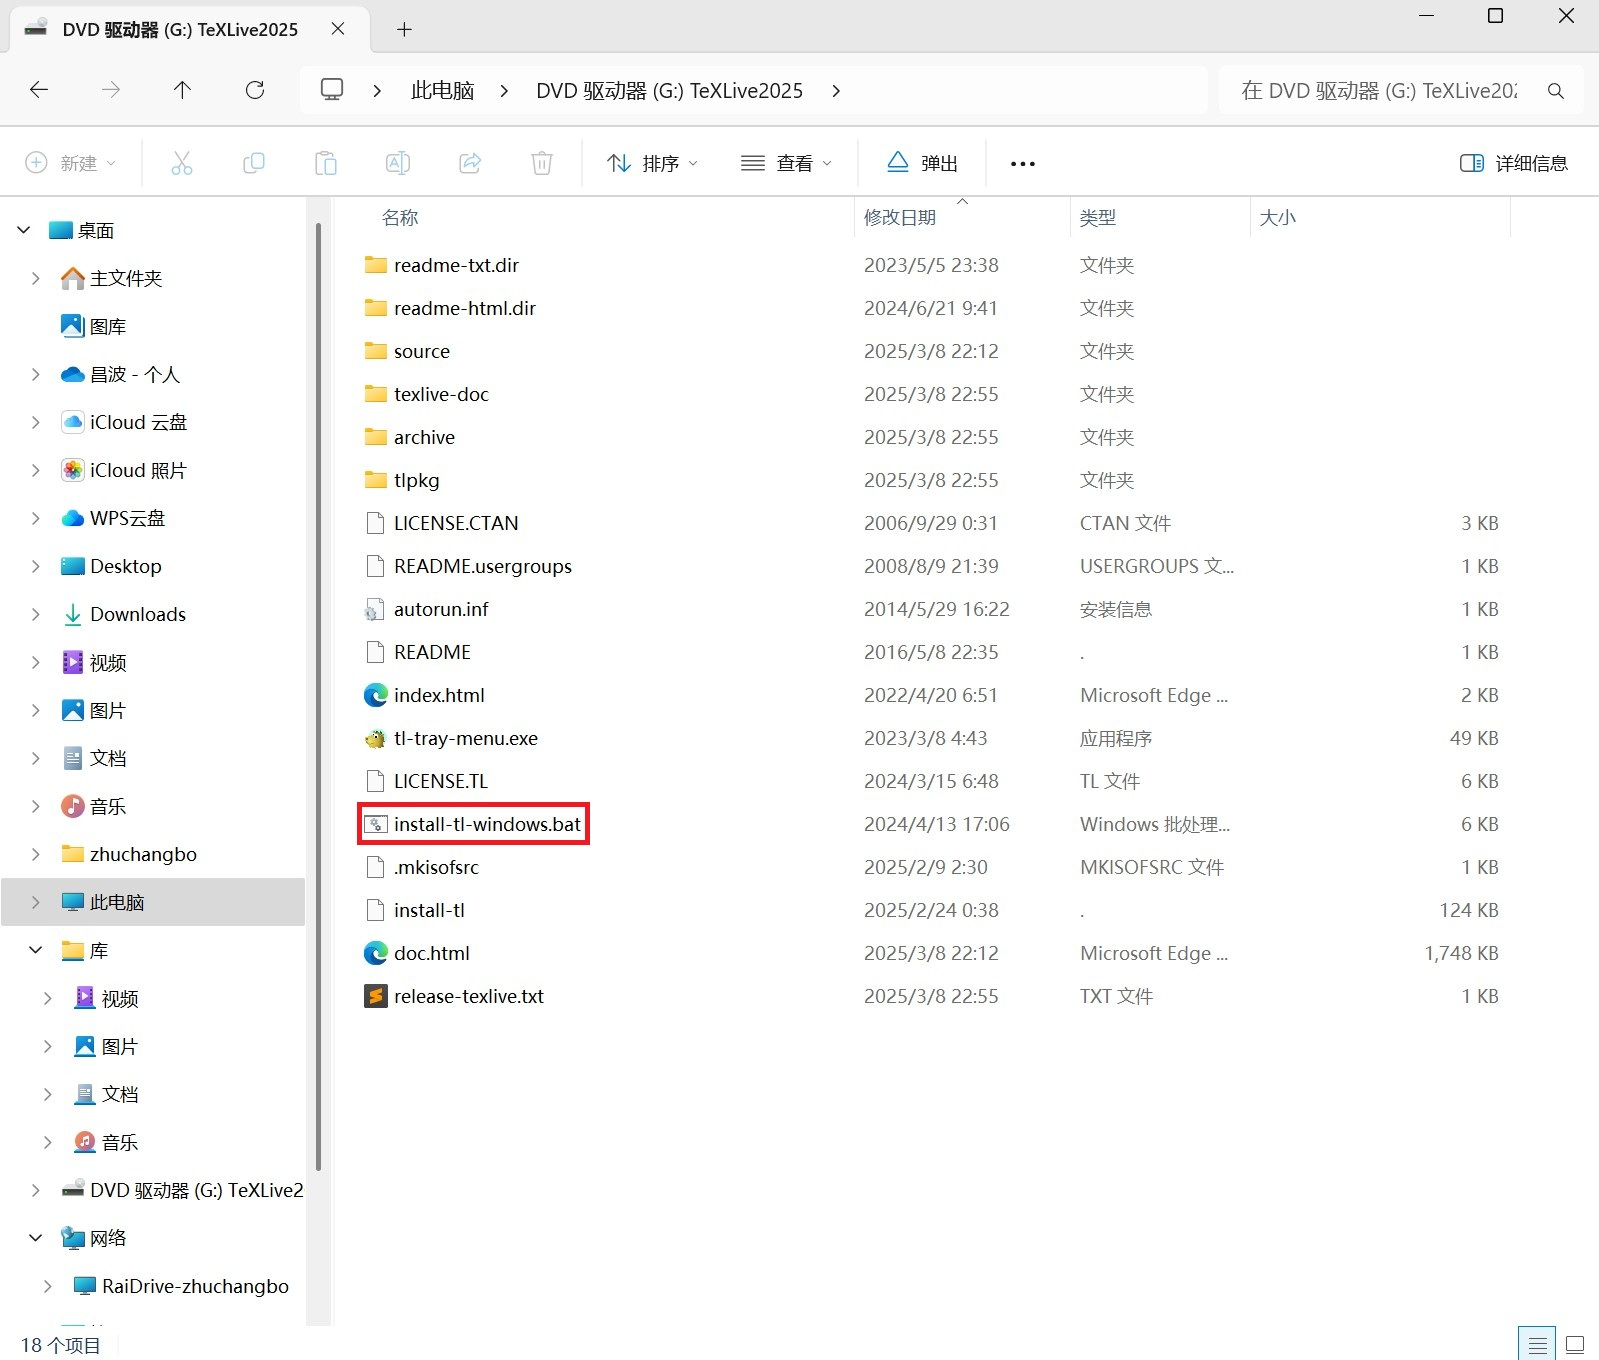
\includegraphics[width=0.8\textwidth]{doc/figures/texlive-iso-content.jpg}
        \caption{\TeX~Live-2025目录}
        \label{fig:texlive-iso-content}
        \end{figure}
\begin{enumerate}
    \item \emph{安装软件}:
        根据所用操作系统和章节~\ref{sec:system}中的信息安装\LaTeX{}编译环境。下面基于windows 11演示安装\TeX~Live和vscode/TeXstudio。\TeX~Live的详细安装教程参见:\href{https://texdoc.org/serve/texlive-zh-cn.pdf/0}{texlive-zh-cn.pdf}(\url{https://texdoc.org/serve/texlive-zh-cn.pdf/0})或者\href{https://github.com/OsbertWang/install-latex-guide-zh-cn}{install-latex-guide-zh-cn}(https://github.com/OsbertWang/install-latex-guide-zh-cn)。
        

        第一步,下载\TeX~Live的ISO镜像文件。国内比较方便的下载站点有 \href{https://mirrors.tuna.tsinghua.edu.cn}{清华大学tuna镜像站}(\href{https://mirrors.tuna.tsinghua.edu.cn/CTAN/systems/texlive/Images/texlive.iso}{点击下载texlive.iso})、\href{https://mirror.nju.edu.cn}{南京大学开源镜像站}(\href{https://mirror.nju.edu.cn/CTAN/systems/texlive/Images/texlive.iso}{点击下载texlive.iso})、\href{https://mirrors.ustc.edu.cn}{中科大开源镜像站}(\href{https://mirrors.ustc.edu.cn/CTAN/systems/texlive/Images/texlive.iso}{点击下载texlive.iso})等等。下载完成后,如图\ref{fig:texlive-iso-content},直接点击下载的文件“texlive.iso”,进入texlive目录。
        

        第二步,以管理员身份运行图\ref{fig:texlive-iso-content}中的批处理文件“install-tl-windows.bat”(shell脚本install-tl是包括Linux系统在内的类unix系统运行的安装文件),在弹出的如图\ref{fig:texlive-tl-gui}所示界面中点击左下角“Advanced(高级)”按钮,可进行相关参数配置。
        \begin{figure}[!hptb]
        \centering
        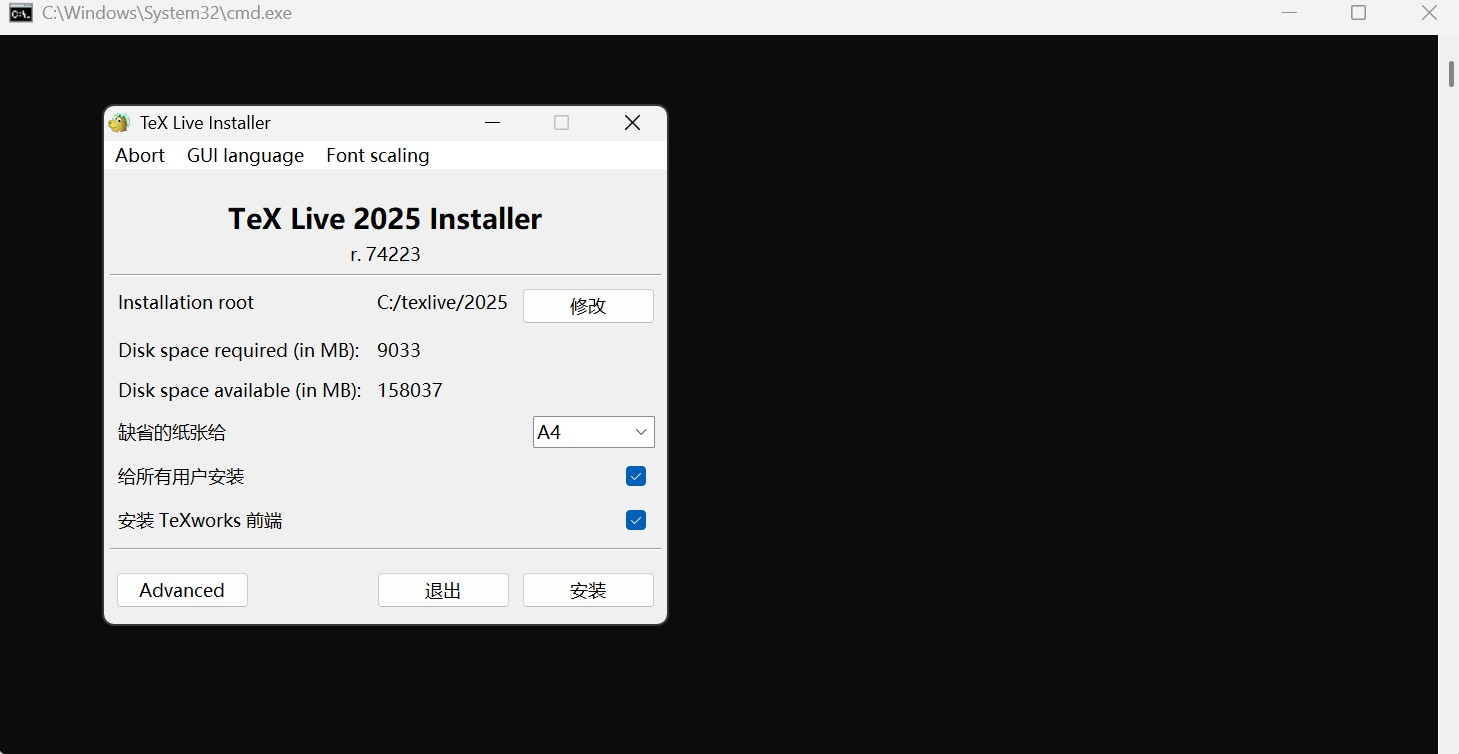
\includegraphics[width=0.8\textwidth]{doc/figures/texlive-tl-gui.jpg}
        \caption{\TeX~Live-2025安装界面}
        \label{fig:texlive-tl-gui}
        \end{figure}

        第三步,如图\ref{fig:texlive-tl-gui-adv},指定三个TDS树目录:
        \begin{itemize}
            \item TEXDIR: 安装根目录,指定TEXMFMAIN树所在目录,例如“C:/texlive”;
            \item TEXMFLOCAL: 指定TEXMFLOCAL树所在目录,系统管理员用来安装供整个系统使用的额外的或更新过的宏包、字体等的目录树,以避免TeX 系统升级等原因而受到影响;
            \item TEXMFHOME: 用户用来安装供他们自己独立使用的的额外的或更新过的宏包、字体等的目录树。这个变量根据不同的用户选择不同的个人目录,例如“\~/texmf”。
        \end{itemize}
        其它选项一般保持默认配置即可。
        \begin{figure}[!hptb]
        \centering
        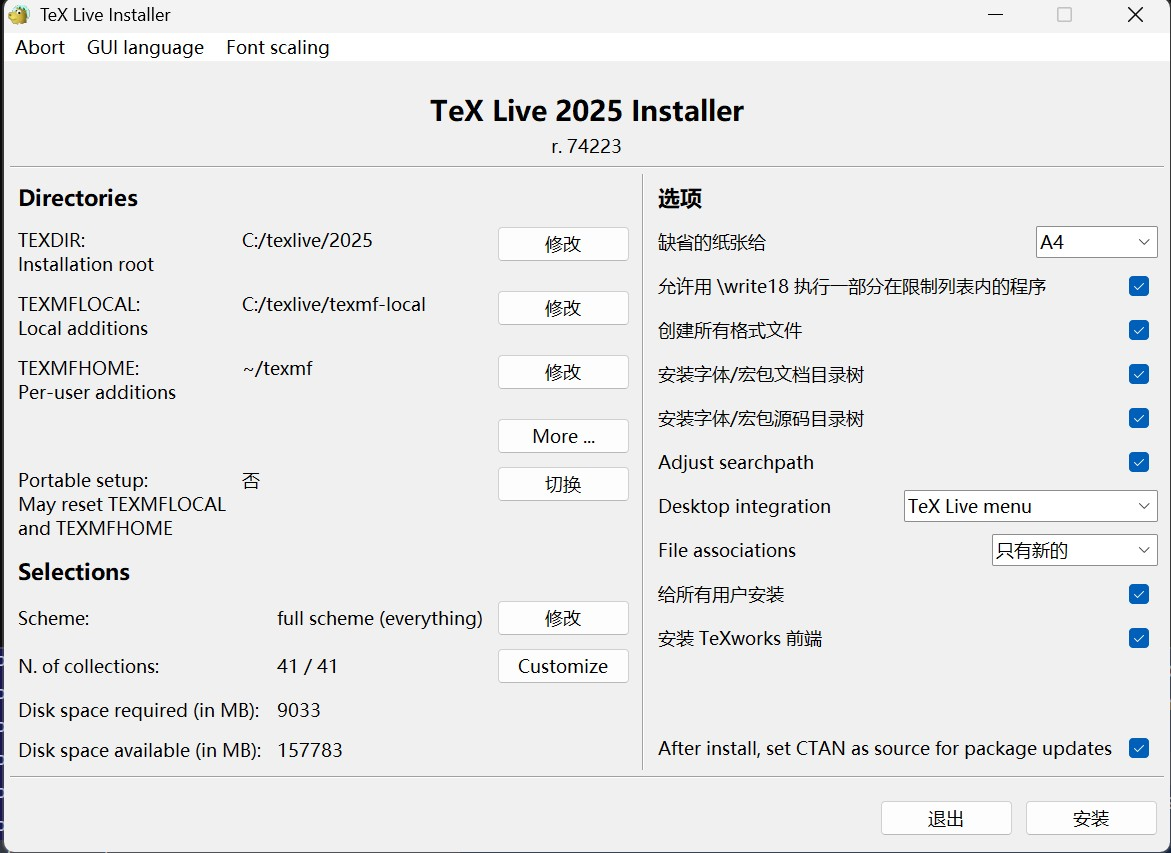
\includegraphics[width=0.8\textwidth]{doc/figures/texlive-tl-gui-adv.jpg}
        \caption{\TeX~Live-2025高级配置界面}
        \label{fig:texlive-tl-gui-adv}
        \end{figure}
        
        第四步,点击图\ref{fig:texlive-tl-gui-adv}右下角所示的“安装”按钮开始安装。直到安装完成,点击“完成”即可。

        第五步,安装TeXstudio。首先\href{https://mirrors.tuna.tsinghua.edu.cn/github-release/texstudio-org/texstudio/LatestRelease/texstudio-4.8.8-win-qt6-signed.exe}{下载TeXstudio},然后,点击“texstudio-4.8.8-win-qt6-signed.exe”进行安装即可。也可以通过\href{https://texstudio.sourceforge.net/}{texstudio官网}(\url{https://texstudio.sourceforge.net/})下载最新版本安装。

        第六步,安装vscode。首先\href{https://vscode.download.prss.microsoft.com/dbazure/download/stable/488a1f239235055e34e673291fb8d8c810886f81/VSCodeUserSetup-x64-1.102.3.exe}{下载vscode},也可以访问\href{https://code.visualstudio.com/Download}{vscode网站}(\url{https://code.visualstudio.com/Download})下载最新版本。然后点击下载的文件进行安装。

    \item \emph{获取模板}:
        下载 \href{https://github.com/changbozhu/\projectname}{\projectname} 模板并解压。 \projectname 模板不仅提供了相应的类文件,同时也提供了包括参考文献等在内的完成中文论文的一切要素,所以,下载时,推荐下载整个 \projectname 模版文件夹,而不是单独的文档类。

        当然,也可以通过git命令克隆仓库到本地: 
        
        \texttt{git clone https://github.com/changbozhu/\projectname.git}
       
    
    \item \emph{基于TeXstudio编译文档}:
        TeXstudio是集成度较高的\LaTeX{}开发编辑器。本部分简单介绍TeXstudio编译本模版的方法。
        
        第一步,打开TeXstudio,在菜单栏打开“选项”->“设置TeXstudio”。如图\ref{fig:texstudio-setup}所示,把“默认编译器”调整为“PdfLaTeX”,“默认文献工具”调整为“Biber”。然后选择右下角的“确定”。
        \begin{figure}[!hptb]
            \centering
            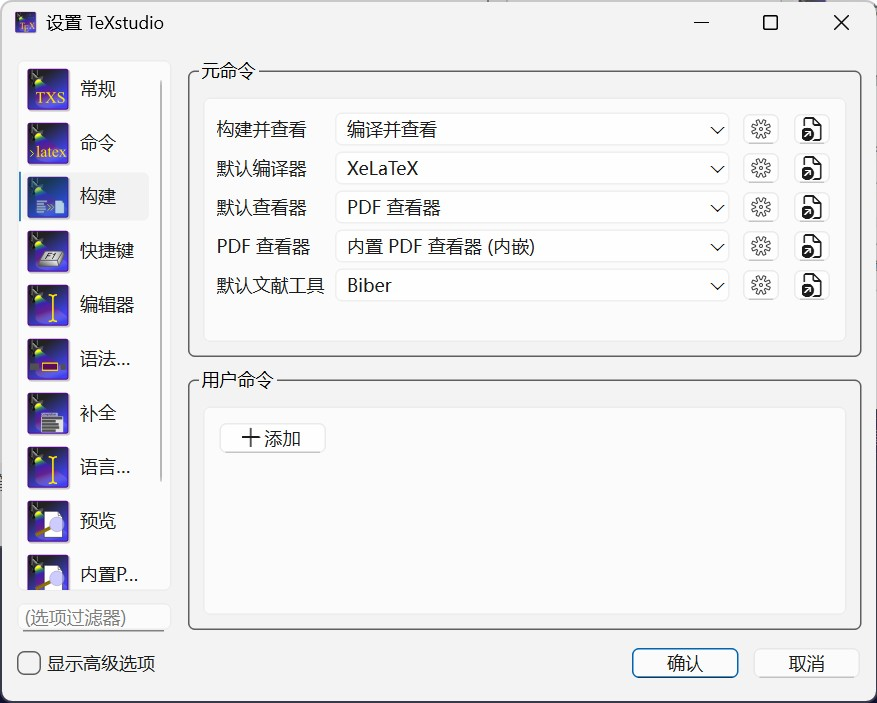
\includegraphics[width=0.6\textwidth]{doc/figures/texstudio-setup.jpg}
            \caption{TeXstudio设置界面}
            \label{fig:texstudio-setup}
        \end{figure}

        第二步,在TeXstudio菜单中打开“文件”->“打开”,出现文件浏览器后导航到模版目录,选择并打开文件“\projectname.tex”,如图\ref{fig:texstudio-doc}所示。
        \begin{figure}[!hptb]
            \centering
            \includegraphics[width=0.6\textwidth]{doc/figures/texstudio-\projectname.jpg}
            \caption{TeXstudio打开文档并构建}
            \label{fig:texstudio-doc}
        \end{figure}

        第三步,如图\ref{fig:texstudio-doc}所示,点击红色框内的绿色按钮,构建并查看文档。
    
    \item \emph{基于vscode编译文档}:
    
 		第一步,打开vscode,如图\ref{fig:vscode-ext}所示,点击左侧栏的“扩展”(如图所示的红色框区域),在图所示的蓝色框搜索区域搜索“Chinese”,在搜索结果中选择“Chinese (Simplified) Language Pack for Visual Studio Code”插件安装。接着搜索“latex workshop”,选择第一个LaTeX Workshop插件进行安装。安装完成后重启vscode。
 		\begin{figure}[!hptb]
            \centering
            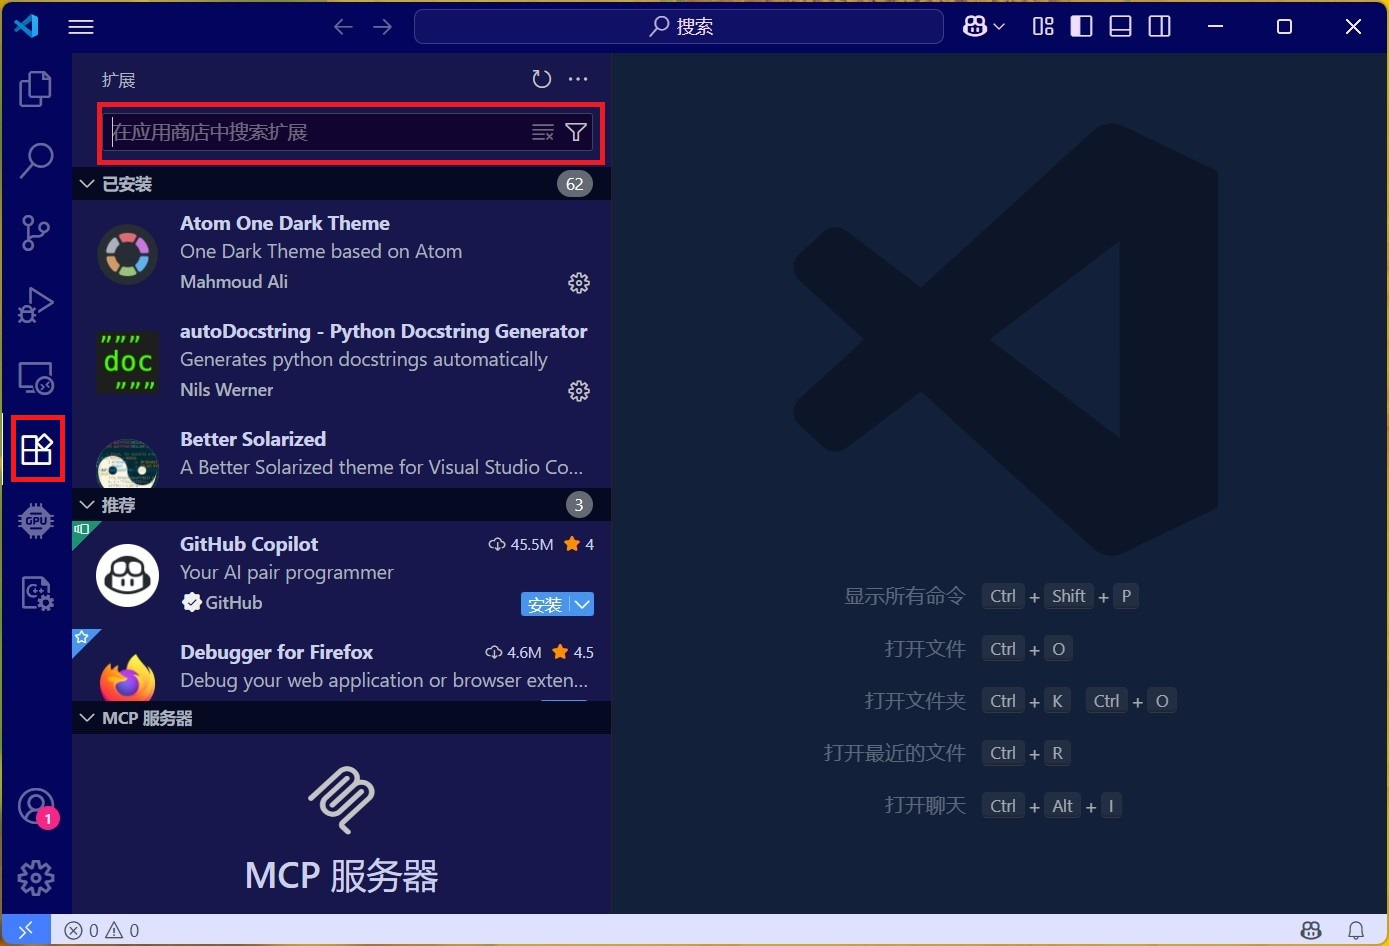
\includegraphics[width=0.8\textwidth]{doc/figures/vscode-ext.jpg}
            \caption{vscode安装插件}
            \label{fig:vscode-ext}
        \end{figure}

 		第二步,点击菜单栏“文件”->“打开文件夹”,在弹出的浏览器窗口选择模版所在文件夹并打开。如图\ref{fig:vscode-openfile}所示,选择左侧边栏最上边的的“资源管理器",可以查看模版文件夹内全部文件,打开”\projectname.tex“,左侧边栏出现”\TeX“字样按钮,点击这个”\TeX“字样按钮。
        \begin{figure}[!hptb]
            \centering
            \includegraphics[width=0.8\textwidth]{doc/figures/vscode-open\projectname.jpg}
            \caption{在vscode中打开文档}
            \label{fig:vscode-openfile}
        \end{figure}

        第三步,展开“构建LaTeX项目”,如图\ref{fig:vscode-buildfile}所示。点击“配方:xelatex->biber->xelatex->xelatex”编译生成文档。
        \begin{figure}[!hptb]
            \centering
            \includegraphics[width=0.8\textwidth]{doc/figures/vscode-build\projectname.jpg}
            \caption{在vscode构建文档}
            \label{fig:vscode-buildfile}
        \end{figure}

        第四步,如图\ref{fig:vscode-pdfview}所示,点击“查看LaTeX PDF”。
 		\begin{figure}[!hptb]
            \centering
            \includegraphics[width=0.8\textwidth]{doc/figures/vscode-\projectname-pdf.jpg}
            \caption{在vscode查看文档}
            \label{fig:vscode-pdfview}
        \end{figure}
 		

    \item \emph{基于命令行编译文档}:
        \begin{enumerate}
            \item Windows:双击运行builder.bat脚本。
            \item Linux或MacOS: {\scriptsize \verb|terminal| -> \verb|chmod +x ./builder.sh| -> \verb|./builder.sh xa \projectname|}
            \item 任意系统:都可使用\LaTeX{}编辑器打开 \projectname.tex文件并选择xelatex编译引擎进行编译。
        \end{enumerate}
    \item \emph{错误处理}:若编译中遇到了问题,请先查看“常见问题”(章节~\ref{sec:qa})。
\end{enumerate}

编译完成即可获得本PDF说明文档。而这也完成了学习使用 \projectname 撰写论文/书籍/报告的一半进程。什么?这就学成一半了,这么简单???,是的,就这么简单!

\section{文档目录简介}

\subsection{文档根目录}

\projectname.tex为主文档文件,默认是本模板的说明文档主文件,也作为样例供用户参考。\projectname.tex供用户定义自己的论文。主文档设计和规划了论文的整体框架,通过对其阅读可以了解整个论文框架的搭建。


\begin{enumerate}
    \item \projectname.tex: 主文件样例,用户文档主文件。
    \item ref.bib:参考文献信息库。
    \item builder.sh: linux/macos下的shell编译脚本。
    \item builder.bat: windows下的dos编译脚本。
    \item usercustom.sty: 用户自定义命令接口。
\end{enumerate}

\subsection{编译脚本}

\begin{itemize}
    \item Windows:双击Dos脚本builder.bat可得全编译后的PDF文档,其存在是为了帮助不了解\LaTeX{}编译过程的初学者跨过编译这第一道坎,请勿通过邮件传播和接收此脚本,以防范Dos脚本的潜在风险。
    \item Linux或MacOS:在terminal中运行
        \begin{itemize}
            \item \verb|./builder.sh xa <mainfilename>|:获得全编译后的PDF文档
            \item \verb|./builder.sh x <mainfilename>|:快速编译,不会生成文献引用
        \end{itemize}
\end{itemize}

全编译指运行 \verb|xelatex+bibtex+xelatex+xelatex| 以正确生成所有的引用链接,如目录,参考文献及引用等。在写作过程中若无添加新的引用,则可用快速编译,即只运行一遍\LaTeX{}编译引擎以减少编译时间。

\subsection{Tmp文件夹}

运行编译脚本后,编译所生成的文档皆存于Tmp文件夹内,包括编译得到的PDF文档,其存在是为了保持工作空间的整洁,因为好的心情是很重要的。

\subsection{style文件夹}

包含ntuthesis文档类的定义文件和配置文件,GB/T 7714引用样式,通过对它们的修改可以实现特定的模版设定。

\begin{enumerate}
    \item \projectname.cls:文档类定义文件,论文的最核心的格式即通过它来定义的。
    \item \projectname.cfg:文档类配置文件,设定如目录显示为“目~录”而非“目录”。
    \item cnbasesetup.sty:常用宏包及文档设定,如字体族、参考文献样式、文献引用样式等。
    \item \projectname setup.sty:设置文档类中一些命令、环境、页眉页脚等”。
\end{enumerate}

\subsection{mlstyle文件夹}
包含用户自定义的机器学习样式文件,如数学样式、神经网络绘图样式、贝叶斯智能体绘图样式等。
\begin{enumerate}
    \item mlmath.sty: 定义了数学基本符号规范,加强了机器学习相关的数学表达式。
    \item bayesianagent.sty: 定义了贝叶斯智能体的一些绘图命令。
    \item deeplearningplot.sty: 定义了深度学习的一些绘图命令,待开发。
    \item snnplot.sty: 定义了脉冲神经网络的一些绘图命令,待开发。
\end{enumerate}

\subsection{doc文件夹}
文件夹内为用户文档的所有实体内容,正常情况下,用户无需修改本文件夹。


\subsection{figures文件夹}
文件夹位默认图片存放与搜索位置,用户可将图片存放于此位置,支持格式有:.jpg, .png, .pdf。不建议为各章节图片建子目录,即使图片众多,若命名规则合理,图片查询亦是十分方便。

\subsection{ \projectname 文件夹}
文档几个模块的基本信息,如论文信息、主内容信息、附录信息等 \footnote{对于研究生学位论文,此文件夹为 \projectname;对于本科生学位论文,此文件夹为 ntudesign 文件夹。}。
\begin{itemize}
    \item FrontBookinfo.tex:为论文信息。
    \item Frontmatter.tex:为论文前序内容。
    \item Mainmatter.tex:列出需要出现的Chapter。写论文时,可以只列出当前章节,以快速编译查看,当论文完成后,再对所有章节进行索引即可。
    \item Appendix.tex:为附录内容。
    \item Backmatter.tex:为论文作者简介和致谢部分等。
\end{itemize}

\subsection{chapters文件夹}
文件夹内为论文的所有实体内容,正常情况下,这也是\textbf{使用 \projectname 撰写论文/书籍/报告时,主要关注和修改的一个位置,注:所有文件都必须采用UTF-8编码,否则编译后将出现乱码文本},\textbf{添加新章时,可拷贝一个已有的章文件再重命名,以继承文档的 UTF8 编码}。

\section{导言区配置 \projectname 文档}
在文档导言区,通过下列命令引入 \projectname.cls文档类、配置几个重要的设置宏包,具体配置的详细信息请参见第\ref{cha:clscfg}章。
\begin{lstlisting}[language=tex]
\documentclass[doctor,academic]{style/ntuthesis}
%\documentclass[twoside,doctor,academic]{style/ntuthesis}
%- Multiple optional arguments:
%- [<oneside|twoside|null>]% oneside print, twoside print, or without print
%- [fontset=<adobe|none|...>]% specify font set instead of automatic detection
%- [scheme=plain]% thesis writing of international students
%- [draft]% show draft version information
%- [standard options for ctex book class: draft|paper size|font size|...]%
%---------------------------------------------------------------------------%
%->> Document settings
%---------------------------------------------------------------------------%

\usepackage[super,color,math,tikz,list,table]{style/cnbasesetup}% document settings
%\usepackage[authoryear,list]{style/cnbasesetup}% document settings
%- usage: \usepackage[option1,option2,...,optionN]{setcnbook}
%- Multiple optional arguments:
%- [bibauto|bibtex|biber]% set bibliography processor and package
%- [<numbers|super|authoryear>]% set citation and reference style
%   - <numbers>: textual: Jones [1]; parenthetical: [1]
%   - <super>: textual: Jones superscript [1]; parenthetical: superscript [1]
%   - <authoryear>: textual: Jones (1995); parenthetical: (Jones, 1995)
%
%- [lscape]% provide landscape layout environment
%- [color]% provide color support via xcolor package
%- [tikz]% provide complex diagrams via tikz package
%- [table]% provide complex tables via ctable package
%- [list]% provide enhanced list environments for algorithm and coding
%- [math]% enable some extra math packages
%- [xlink]% disable link colors


\usepackage{style/ntuthesissetup}% document settings
\usepackage{mlstyle/mlmath}% extension to amsmath
\usepackage{mlstyle/bayesianagent}
% user defined commands
\usepackage{usercustom}
%\addbibresource{ref.bib} % only for biber



%设置固定\normalbaselineskip行距的字体
% 包括 \chuhao \xiaochu \yihao \xiaoyi \erhao \sanhao \sihao \wuhao \liuhao
\xiaosi
%\baselineskip = \linespread * \normalbaselineskip
%
%


%-> Titlepage information
%-
%---------------------------------------------------------------------------%
%->> School information
%-  不建议用户修改此处
\schoollogo[width=8.16cm,height=2.34cm]{official/ntu/ntu-logo}% 校名logo  不要修改
\schoolbadge[width=3.78cm,height=3.78cm]{official/ntu/ntu-badge}% 校徽    不要修改

%---------------------------------------------------------------------------%
%->> Tehsis Structure information
% 
%-->> 学位类别
%-限填医学博士、工学博士、文学硕士、理学硕士、医学硕士、临床医学专业硕士等
\degree{工学博士}% 

\classid{TP391.4}

%-->>是否涉密
%-
% 学位论文是否涉密,不涉密不要启用此命令,已做默认不涉密配置
% 对于涉密的学位论文,第一个参数指定为'yes',第二个参数为阿拉伯数字,指定保密年限,
% \confidential{yes|no}{period}
% 例如保密2年的学位论文:
%\confidential{yes}{2}


%---------------------------------------------------------------------------%
%->> Titlepage information
%---------------------------------------------------------------------------%
%-
%-> 个人中英文信息
%-

% 标题
  %   可使用“\\”命令手动控制换行
  %   如:\title{脉冲神经网\\高效学习理论研究}
\title{南通大学学位论文 \LaTeX{}模板 V\projectversion}% 论文中文题目
\title*{Nantong University Thesis \LaTeX{} Template V\projectversion}% English title

% 作者
%   作者姓名需要与学籍信息一致
\author{朱昌波}% 论文作者
\author*{Changbo Zhu}%English
% 学号
%   学号需要与学籍信息一致
\studentid{202100111002}% 学生学号

% 指导教师
%   指导教师需要与学籍信息一致
\advisor{X**~教授}% 指导教师:姓名 专业技术职务 工作单位
\advisor*{Prof.~** X}% 指导教师:姓名 专业技术职务 工作单位

%联合指导教师,如果没有,请清空内容或注释命令
\coadvisor{Y**~副教授}
\coadvisor*{Assoc. Prof.~** Y}


% 专业
%   填写学籍信息中专业的全名及代码
\major{模式识别与智能系统}% 一级/二级学科专业名称,专业名称需要与学籍信息一致
\major*{Pattern Recognition and Intelligent Systems}
\majorcode{081104}% 一级/二级学科专业代码,专业名称需要与学籍信息一致

\researchfield{认知神经计算}
%
% 培养单位
%   填写所属院系的全名
\department{XXXXXX学院}% 院系名称
%\department{电气工程与自动化学院\\神经网络与智能机器人研究所}% 多行院系名称示例

% 论文完成日期
% \completedate{<year>}{<month>}{<date>}
\completedate{二〇二五}{九}{一}% 

\foundation{××科学基金(30000000)\\××科学研究基金(WKJ2008-0-000)}



%
\end{lstlisting}

如果用户有自定义命令,可以写入样式宏包usercustom.sty内。默认的参考文献处理器为 `bibauto` 模式,实际后台默认调用biber(biblatex),文献库文件默认为“ref.bib”。 命令 \verb|\xiaosi| 设置默认字号为行固定间距的小四号字体。文件“ntuthesis/Frontinfo.tex”配置了学位论文相关信息。

\section{文档主体内容}
位于 \verb|\begin{document}|和 \verb|\end{document}| 之间的内容均是文档主体内容。
\begin{lstlisting}[language=tex]
\begin{document}
%-> 生成扉页、原创性声明、授权声明、标题页中英文摘要
\maketitle% cover and titlepage,
\tableofcontents

%-> Frontmatter:  abstract, content list, symbol list, preface
\frontmatter% initialize the environment
%---------------------------------------------------------------------------%
%->> Frontmatter
%-

%---------------------------------------------------------------------------------------------------------------
%-> 摘要
%-
%- 摘要内容要求在800~1200字,应简要说明本论文的目的、方法、结果和结论。
%- 要突出论文的创新之处。语言力求精炼、准确。在本页的最下方另起一行,
%- 注明本文的关键词(3-5个)。
%- 摘要内容要求在800~1200字,应简要说明本论文的目的、方法、结果和结论。
%- 要突出论文的创新之处。语言力求精炼、准确。在本页的最下方另起一行,
%- 注明本文的关键词(3-5个)。
%摘要是以提供文献内容梗概为目的,不加评论和补充解释,简明、确切地记述文献重要内容的短文。其要素一般包括:
% -(1)目的——研究、研制、调查等的前提、目的和任务,所涉及的主要范围;
% -(2)方法——所用的原理、理论、条件、对象、材料、工艺、结构、手段、装备、程序等;
% -(3)结果——实验的、研究的结果,数据,被确定的关系,观察结果,得到的效果,性能等;
% -(4)结论——结果的分析、研究、比较、评价、应用,提出的问题,今后的课题,假设,启发,建议,预测等; 
%
%写摘要时不得简单地重复题名中已有的信息,要排除在本学科领域中已成常识的内容,要用第三人称的写法。
%应采用“对……进行了研究”、“报告了……现状”、“进行了……调查”等记述方法,不使用“本文”、“作者”等作为主语。
%摘要的第一句不要与题目重复;取消或减少背景信息,只表示新情况、新内容;不说空洞的词句,
%如“本文所讨论的工作是对过去×××的一个极大地改进”、“本工作首次实现了……”、“经检索尚未发现与本文类似的工作”等;
%此外,作者的打算及未来的计划不能纳入摘要。
%
%列出3~5个关键词,以关键字与课题间关联性由强到弱顺序排列,关键词之间用分号相隔,结束处不用标点符号。
\begin{abstract}    
\parwords{目的}  近期,主动推理的机制框架被提出作为发展意识统一理论的原则性基础,有望解决该领域的概念分歧。我们认为,要实现这一愿景,当前基于主动推理框架的提案需进一步完善,以形成真正的意识过程理论。

\parwords{方法}  提升机制性理论的途径之一,是采用计算模型等形式化方法来实现、调适和验证提出的概念框架。本文系统考察了计算建模方法如何助力完善主动推断与意识关联的理论提案,重点关注:(1)这些模型在容纳不同意识维度和实验范式方面的开发广度与成效;(2)如何通过仿真与实证数据检验和改进模型。

\parwords{结果}  尽管当前研究已取得鼓舞人心的成果,但我们认为这些探索仍处于初级阶段。要提升模型的结构效度与预测效度,必须通过未观测的新神经数据进行实证检验。


\parwords{结论}  主动推断要成为完备的意识理论仍面临关键挑战:模型需能解释广泛的意识现象谱系,特别是涵盖经验的现象学特征。尽管存在这些不足,该方法已被证明是推动理论发展的有效路径,为未来研究提供了重要潜力。

\keywords{什么什么,细胞,相关性}
\end{abstract}

%英文摘要上方应有题目,内容与中文摘要相同。
%在英文题目下面第一行写研究生姓名,专业名称用括弧括起置于姓名之后,
%研究生姓名下面一行写导师姓名,格式为Directed by...。
%最下方一行为英文关键词(Keywords 3-5个)
\begin{abstract*}
\parwords*{Purpose}  The abstract serves both as a general introduction to the topic and as a brief, non-technical summary of the main results and their implications. The abstract must not include subheadings (unless expressly permitted in the journal's Instructions to Authors), equations or citations.  Most journals do not set a hard limit however authors are advised to check the author instructions for the journal they are submitting to.

\parwords*{Methods}  The abstract serves both as a general introduction to the topic and as a brief, non-technical summary of the main results and their implications. The abstract must not include subheadings (unless expressly permitted in the journal's Instructions to Authors), equations or citations. Most journals do not set a hard limit however authors are advised to check the author instructions for the journal they are submitting to.

\parwords*{Results}  The abstract serves both as a general introduction to the topic and as a brief, non-technical summary of the main results and their implications. The abstract must not include subheadings (unless expressly permitted in the journal's Instructions to Authors), equations or citations.  Most journals do not set a hard limit however authors are advised to check the author instructions for the journal they are submitting to.


\parwords*{Conclusion} The abstract serves both as a general introduction to the topic and as a brief, non-technical summary of the main results and their implications. The abstract must not include subheadings (unless expressly permitted in the journal's Instructions to Authors), equations or citations.  Most journals do not set a hard limit however authors are advised to check the author instructions for the journal they are submitting to.

\keywords*{Variational Bayesian method, Free energy principle, Cognitive neuroscience}
\end{abstract*}
% title page, abstract

%--> Main matter: 
\mainmatter
%-----------------------------------------------------------------%
%->> Main content
%-----------------------------------------------------------------%

\chapter{绪论} \label{chap:review}
\section{课题来源、研究的目的和意义} \label{sec:review:purpose}

临床上,慢性疼痛是一类发病率很高的疾病,大约占成年人群的30\%。全世界每年用于疼痛治疗的费用高达数千亿美元,目前临床上使用的镇痛手段对神经病理性疼痛和癌症痛等顽固性疼痛的疗效非常有限,迫切需要开发新的更为有效的治疗手段。因此,痛觉研究成为神经科学的前沿课题之一。


\section{国内外研究概况}\label{sec:review:current}
\subsection{国外研究概况}\label{subsec:review:current:foreign}
临床上,慢性疼痛是一类发病率很高的疾病,大约占成年人群的30\%。全世界每年用于疼痛治疗的费用高达数千亿美元,目前临床上使用的镇痛手段对神经病理性疼痛和癌症痛等顽固性疼痛的疗效非常有限,迫切需要开发新的更为有效的治疗手段。因此,痛觉研究成为神经科学的前沿课题之一。

\begin{enumerate}
\item 加拿大的… …。
\item … …
\end{enumerate}


\subsection{国内研究概况}\label{subsec:review:current:domestic}
国内还没看到相关方面的报道… …现在所通用的NC代码 \cite{vossel_spatial_2014} ……



\section{论文的主要研究内容}\label{sec:review:research}
本论文是以作者攻读硕士学位期间承担课题的工作为基础,…


\chapter{材料与方法} \label{chap:materials}
\section{研究资料及仪器设备} \label{sec:materials:obj-dev}

... ...

\subsection{研究对象}\label{subsec:materials:obj-dev:obj}
... ...

\subsection{主要仪器与试剂}\label{subsec:materials:obj-dev:dev}

... ...

\section{实验流程与方法}\label{sec:materials:proc-method}
\subsection{标本制作}\label{subsec:materials:proc-method:specimens}
\subsection{获取数据}\label{subsec:materials:proc-method:getdata}
\subsection{分析数据}\label{subsec:materials:proc-method:analysisdata}
\subsection{测定数据}\label{subsec:materials:proc-method:measured data}
\subsection{统计学处理 }\label{subsec:materials:proc-method:statistic}



\chapter{结果} \label{chap:results}




\chapter{结论与展望}\label{chap:conclusion}
\section{论文总结}
本研究的目标是基于贝叶斯脑假设\cite{beal2003VB,Friston_freeEnergy_2010,daunizeau2010observingA,daunizeau2010observingB,Mathys2011HGF}研究动态环境中智能体的感知与学习。本文深入研究了智能体在动态环境中对不确定性的表征及高效学习与决策。研究受到认知神经科学中人类在动态环境下的决策行为及生物神经系统中神经元低阶交互的信息表征机制的启发,在贝叶斯脑假设下,从理论层面构建了不同类型动态环境的概率描述模型,并且智能体内部以一致的层次化方式抽象表征了不同类型动态环境的不确定性。本文中基于不同类型的动态环境构建了一系列的模型及仿真,详尽论述了所构建智能体对动态环境不确定性(波动)的高效感知与表征,并且是可概率描述的动态环境中最优的学习推断模型。这为动态环境下自适应行为的机制提供了一个有前景的最优的概率解释模型。本文主要开展了下述内容的研究:
\begin{enumerate}
	\item {\verb|基于多尺度不确定性表征的感知模型|}:针对一般动态环境中不确定性表征问题,提出了一般层次化布朗滤波,有效解决了动态环境中高斯假设下不确定性的多尺度表征与学习的问题。
	动态环境中的智能体必须具备对环境的不确定性理解与表征的机制。在高斯与布朗运动假设下,环境的时变不确定性被布朗运动的扩散强度矩阵所表征。进一步地,为了提高对环境不确定性表征的灵活性、高效性、时变动态性,扩散强度矩阵被另一个布朗运动参数化表征。以此类推,可构建多层级的布朗运动对环境不确定性(波动)进行多尺度的表征与学习。 
	进一步地,针对一般层次化布朗滤波的反演,基于变分贝叶斯方法整合平均场假设及基于一步牛顿法的高斯二次型近似,提出了一般层次化布朗滤波及其变体模型的反演方案,把推断的优化问题转变为状态的解析更新,简化了模型的逆向推断,提高了推断效率。从而,模型的变分逆被一组高效的、可解析的更新方程所实现。然后,我们在鱼的u-turn轨迹中测试了模型的性能。结果表明,模型很好的捕捉了轨迹的动态特征。
	\item {\verb|基于多元伯努利分布的动态环境不确定性表征与感知学习|}:动态地多元二值环境是神经科学中常用的实验环境。通常使用独立的多元伯努利分布描述多元二值的状态。一方面,如果智能体仅仅使用这个模型描述动态波动的环境,那么便丢失了对环境结构及不确定性的理解能力。另一方面,被伯努利分布所描述的二值环境的全部信息包含在自然参数向量里,这样智能体便可利用层次化布朗滤波跟踪自然参数向量即可。独立的伯努利分布的缺陷也会被低阶交互地自然参数所弥补。为了评估模型在动态波动的二值环境中的感知与决策能力,我们设想了一个双臂赌博任务,并依据贝叶斯决策理论构建了响应模型,与基于层次化的布朗滤波的感知模型共同形成贝叶斯智能体。仿真研究的结果表明,智能体很好的理解了动态波动的二值环境。几乎以最优的方式在二值环境中产生了决策行为。
	\item {\verb|基于指数分布的动态环境不确定性表征与感知学习|}:动态地多元指数分布环境是神经科学中常用的实验环境。通常使用独立的多元指数分布描述环境的状态。一方面,如果智能体仅仅使用这个模型描述动态波动的环境,那么便丢失了对环境结构及率强度参数不稳定波动的理解能力。另一方面,被指数分布所描述的动态环境的全部信息包含在率强度参数向量里,这样智能体便可利用层次化布朗滤波跟踪率强度参数向量的对数即可。独立的指数分布的缺陷也会被低阶交互地率强度参数所弥补。为了研究模型在动态指数分布信号环境中的感知,我们构建了一个动态率强度的仿真任务,模型很好的捕获了动态指数分布信号环境的基本统计特征。进一步地,我们消融了层次化布朗滤波中的波动层,获得了假设外部环境波动为常量的新模型。通过贝叶斯模型选择,消融模型不能很好的表征环境波动而变成次优模型。
	\item {\verb|基于分类分布的动态环境不确定性表征与感知学习|}:为了表征分类分布,我们把其状态固定到一个多元高斯分布空间中考虑,每个状态的概率与其在多元高斯分布内的密度成正比。这样我们便把离散状态的不确定性转换成了多元高斯分布的中心位置及其不确定性。进一步地,我们可以使用层次化布朗滤波跟踪上述多元高斯分布的中心位置及其不确定性。
	为了研究模型在动态分类分布环境中的感知,我们构建了一个动态分类感知的仿真任务,模型很好的捕获了动态分类分布环境的基本统计特征。进一步地,我们消融了层次化布朗滤波中的波动层,获得了假设外部环境波动为常量的新模型。通过贝叶斯模型选择,消融模型不能很好的表征环境波动而变成次优模型。
	\item {\verb|基于不确定性调节的自适应学习率机制|}:为了研究不确定性调节的自适应学习率,文中提出了基于高斯随机游走和伯努利分布的层次化贝叶斯模型,并且其学习率具有基于信念和环境不确定性所调节的自适应机制,能够有效且准确地推断动态二分类环境中的隐概率。在这个层次化贝叶斯模型中,隐状态的更新规则是具有恒定学习率的Rescorla-Wagner更新规则的扩展,即恒定学习率扩展为基于信念和环境不确定性调节的时变自适应学习率。
	作为模型自适应推断的重要机制,受信念和环境不确定性调控的自适应学习率有助于促进对生物自适应行为机制的理解,也为进一步开发新型自适应机器学习模型提供了理论框架。
	本文中基于随机生成的数据验证了学习率自适应机制的有效性和高效性。
\end{enumerate}


本文在贝叶斯脑假设下立足于动态环境中自适应学习模型的构建,结合了神经科学与机器学习,以探索动态环境下不确定性的表征、学习与决策。本项研究的重要任务之一就是探索一般动态环境下的不确定性(波动)的表征机制。这是保障智能体在动态环境下准确认知环境的基础,也是后续动态环境下决策的前提。本项研究的另一个重要任务就是抽象现实世界不同类型的动态环境,并构建相应动态环境下不确定性表征的贝叶斯模型。总之,本项研究内容新颖,具有较高的模型理论前瞻性和创新性,具有较好的应用前景和价值,其主要贡献和研究意义概括如下:
\begin{enumerate}
	\item {\verb|提出了一般层次化布朗滤波|}:受到贝叶斯脑假设下层次化先验信念的表达及神经元集群中成对低阶交互的信息表征机制的启发,基于高斯和布朗假设,构建了层次化的布朗运动以对动态环境不确定性(波动)形成层次化多尺度表征。有效地解决了动态环境中高斯假设下不确定性的多尺度表征与学习问题。
	
	\item {\verb|提出了层次化布朗滤波及其变体模型的解析反演方案|}: 针对一般层次化布朗滤波及其变体模型的反演,提出了一般层次化布朗滤波及其变体模型的变分反演方案, 整合了变分贝叶斯方法、平均场假设和基于一步牛顿法的高斯二次型近似,把较高计算开销的优化问题转变成了低计算开销的状态更新,简化了模型的逆向推断,提高了推断效率。
	
	\item {\verb|提出了动态指数族分布环境下不确定性表征与学习方案|}: 针对动态指数族分布所描述的环境中不确定性感知与学习,提出了基于一般层次化布朗滤波的贝叶斯感知模型,有效解决了指数族分布环境中充分统计量评估及环境不确定性认知的问题,揭示了动态指数族分布环境下不确定性感知的一般机制。
	
	\item {\verb|提出了一种基于不确定性的学习率调节机制|}: 主要针对动态环境下的学习机制问题,有效解决了智能体动态环境下学习率调节与形成问题,提高了智能体对环境的感知效率。总之,基于信念和环境不确定性的学习率自适应调节机制是模型信息处理的标志,也为进一步探讨智能体高效学习模型的构建提供了可借鉴的机制。
	
	
	%\item {\verb|提出了多元动态二值环境的概率描述及相应的层次化贝叶斯感知模型|}:受到社交认知学习实验的启发,我们构建了动态多元二值环境的概率描述。并基于层次化布朗滤波构建了层次化贝叶斯模型,以高效认知动态多元二值环境。同时,在变分贝叶斯和平均场近似下,我们获得了动态多元二值环境中伯努利自然参数和不确定性的高效更新规则。后验期望状态的学习过程被不确定性(波动)所调节。
	%\item {\verb|提出了多元动态指数分布环境的概率描述及相应的层次化贝叶斯感知模型|}:受到脑内信号肥尾特征及泊松过程事件等待时间的启发,我们构建了动态多元指数分布环境的概率描述。并基于层次化布朗滤波构建了层次化贝叶斯模型,以高效认知动态多元指数分布环境。同时,在变分贝叶斯和平均场近似下,我们获得了动态多元指数分布环境中指数分布率强度对数及其不确定性的高效更新规则。后验期望状态的学习过程被不确定性(波动)所调节,呈现出预测编码的更新方式。
	%\item {\verb|提出了多元动态分类分布环境的概率描述及相应的层次化贝叶斯感知模型|}:受到认知实验(如小鼠走迷宫,赢者通吃)的启发,我们构建了动态分类分布环境的概率描述。并基于层次化布朗滤波构建了层次化贝叶斯模型,以高效认知动态分类分布环境。同时,在变分贝叶斯和平均场近似下,我们获得了动态分类分布环境中离散高斯分布的位置及其不确定性的高效更新规则。后验期望状态的学习过程被不确定性(波动)所调节,呈现出预测编码的更新方式。
\end{enumerate}

\section{未来工作展望}
动态环境的认知建模对研究生物适应性行为及解析自适应性行为背后的机制至关重要。动态环境下,智能体需要高效的信息的处理机制,以应对复杂多变的动态环境。本文基于理论层面构建了动态环境下一般层次化布朗滤波。未来还有多个方向可以开展深入研究:
\begin{enumerate}
	\item {\verb|认知实验|}:动态环境的不确定性表征和认知学习是考察生物智能体学习和认知特征的很好环境。依照本文提供的模型进行有针对的实验设计,有望解析出人类在复杂动态环境下的行为机制。
	\item {\verb|神经网络模型|}:一般层次化布朗滤波为我们提供了一个很好的框架。基于这个框架我们可以构建更一般的神经网络模型。探索大脑执行贝叶斯推断的一般机制。
	\item {\verb|自适应信息处理|}: 本文提供了动态环境下不确定性的层次化表征,形成了自适应学习率更新规则。进一步解析动态学习率的调节机制,是下一步很好的研究方向。
\end{enumerate}
%-----------------------------------------------------------------%


%-> Bibliography, glossary, index
%-
%reference matter
{
\intotoc*{\cleardoublepage}{\bibname}% add link to toc
\linespread{1.25}
\ntuthesisbibliography%{ref}
}
\intotoc\chapter*{英文缩略词表}%
\begin{abbreviation}
\addabbrvitem{CFD}{Computational Fluid Dynamics}{计算流体动力学}
\addabbrvitem{VBM}{Variational Bayesian Method}{变分贝叶斯方法}
\addabbrvitem{VBM}{Variational Bayesian Method}{变分贝叶斯方法测试赛测磁海带丝大萨达咔哒扩大凯撒卡拉季巅峰对决分开发进度款}
\addabbrvitem{VBM}{Variational Bayesian Method}{变分贝叶斯方法测试赛测磁海带丝大萨达咔哒扩大凯撒卡拉季巅峰对决分开发进度款}
\end{abbreviation}



%------------------------------------------------------------------
%- 不需要综述的,请注释下面一行代码

%-
%-
% Reviews and References
%---------------------------------------------------------------------------%
%->> Reviews
%---------------------------------------------------------------------------%
\begin{review}
学位论文为了需要反映出作者确已掌握了坚实的基础理论和系统的专门知识,具有开阔的科学视野,对研究方案作了充分论证,因此,有关历史回顾和前人工作的综合评述,以及理论分析等,应单独成章,用足够的文字叙述。

综述参考文献引用测试
\cite{berger2013statistical,carpenter2022_game,feynman1972statistical}
\end{review}


%-> 附录
\appendix
%---------------------------------------------------------------------------%
%->> Main content
%---------------------------------------------------------------------------%
\chapter{南通大学学位论文格式要求}\label{appendix:ntuthesisrule}

研究生学位论文是研究生科学研究工作的全面总结,是描述其研究成果、代表其研究水平的重要学术文献资料,是申请和授予相应学位的基本依据。为规范我校博士、硕士学位论文形式,按照国家标准局颁布的《科学技术报告、学位论文和学术论文的编写格式》,结合我校实际情况,特制定本要求。

\section{学位论文字数要求}
研究生学位论文一般用中文撰写(特殊专业除外)。撰写学位论文应简明、扼要,既能够全面、真实反映个人的研究工作,达到相应申请学位水平,又不能抄袭或搬用别人的研究成果或理论(正常的引用除外,但需注明出处,且引用不宜篇幅过长)。学位论文字数可由学院根据学科特点以及专业(领域)相应的全国教育指导委员会要求自行规定,但不能低于学校规定的最低标准。学位论文字数(不包括图表)要求:
\begin{enumerate}
\item 自然科学类博士学位论文一般不少于5万字;
\item 自然科学类学术学位硕士学位论文一般不少于3万字,人文社科类学术学位硕士学位论文一般不少于4万字;
\item 专业学位硕士研究生学位论文字数要求由校专业学位研究生培养指导委员会根据各专业学位类别相应的全国教育指导委员会要求制定。
\end{enumerate}

\section{学位论文内容及编排顺序}
\begin{enumerate}
\item 封面
\item 学位论文原创性声明及使用授权声明
\item 扉页
\item 目录
\item 中英文摘要
\item 绪论
\item 正文
\item 结论或结语
\item 参考文献
\item 文献综述
\item 附录
\item 攻读学位期间取得的成果
\item 致谢
\end{enumerate}
如无法被上述部分囊括的,可自酌设定后,插入适当位置。

\section{学位论文各部分格式要求}
详见研究生院网站下载中心-\href{https://yjs.ntu.edu.cn/2024/1009/c7679a250968/page.htm}{\emph{南通大学博硕士学位论文格式模板(2024版)}}。

\section{论文印刷及装订要求}
\begin{enumerate}
\item 论文封面采用皮纹纸,全校统一格式。同时需要调整封面颜色为:\emph[crimson]{博士学位论文的封面为深红色},\emph{学术学位硕士学位论文封面为白色},\emph[light-green]{专业学位硕士论文封面为浅绿色}。
\item 双面打印,胶装。纸张方向:纵向;除封面外,所有页面边界为,上3.8厘米,下3.8厘米,左3.2厘米,右3.2厘米;页眉2.8厘米,页脚2.6厘米。对齐方式:两端对齐;首行缩进0.92厘米或2字符;行间距:固定值20磅。打印论文装订后的尺寸为285mm×205mm(版心尺寸为240mm×150mm)。
\end{enumerate}

\parwords{论文无附录者无需附录部分}
\parwords{论文无综述者无需综述及综述参考文献}

\chapter{ 南通大学本科毕业设计(论文)学术不端行为处理办法(试行)}

为进一步提高本科毕业论文(设计)质量,加强学术道德和学风建设,营造诚信学术氛围,推动广大本科生科学引用文献资源,规范本科毕业设计(论文)管理,根据教育部《关于树立社会主义荣辱观进一步加强学术道德建设的意见》、《关于严肃处理高等学校学术不端行为的通知》、《学位论文作假行为处理办法》等有关文件精神和《南通大学学术不端行为处理规程(试行)》(通大〔2012〕32号)等文件规定,防范和处理本科毕业设计(论文)学术不端行为,特制订本办法。 

第一条 \quad 本办法适用于本科毕业设计(论文),本科生应严格遵守学术规范,恪守学术道德,弘扬优良学风,在指导教师指导下独立完成毕业设计(论文)。出现毕业设计(论文)学术不端行为的,学校将按本办法对当事人进行处理。 

第二条 \quad 本科毕业设计(论文)学术不端行为包括以下情形:
\begin{enumerate}
    \item 购买、出售毕业设计(论文)或组织毕业设计(论文)买卖的;由他人代做、为他人代做毕业设计(论文)或者组织毕业设计(论文)代做的。
    \item 使用他人已发表的数据、图表等内容未经授权或未注明出处的。 
    \item 照搬他人论文或著作中的实验结果及分析、系统设计和问题解决办法而没有注明出处或未说明借鉴来源的。
    \item 有过度引用行为的。引用他人内容已按规范注明出处,但文字复制比超过$30\%$的为抄袭,文字复制比大于$50\%$的为严重抄袭。
    \item 伪造数据的。 
    \item 有其他毕业设计(论文)学术不端行为的。
\end{enumerate}

第三条 \quad 学校将加强学术诚信建设,建立毕业设计(论文)学术诚信检查制度,每年在答辩前对本科毕业设计(论文)统一进行学术诚信审查和抄袭检测,检测结果作为毕业设计(论文)学术不端行为的基本认定依据。 

第四条 \quad 学术不端行为的认定和处理 
\begin{enumerate}
    \item 对举报或检查发现毕业设计(论文)有学术不端行为情形,学校将组织有关人员对其进行调查认定。经查实确认有上述学术不端行为的,由相关学院对论文作者进行批评教育、责令改正,并视情节轻重责令其修改论文、重新撰写论文、推迟答辩、取消学位(毕业)申请(答辩)资格等处理;已经获得学历学位的,依法撤销所获学位,注销所获学历证书。 
    \item 对于出现剽窃、抄袭等学术不端行为的学生,学校将依据《南通大学学生纪律处分规定》进行处理;对于为他人代做、出售毕业设计 (论文)或者组织毕业设计 (论文)买卖、代做的学生,按《南通大学学术不端行为处理规程(试行)》(通大〔2012〕32号)给予相应处理。 
    \item 对论文学术不端行为当事人做出处理决定前,学校将告知并听取当事人的陈述和申辩。当事人对处理决定如有异议的,可以在收到处理决定之日起5个工作日内向校学风建设领导小组提出书面申诉。对当事人提出的申诉,学校予以组织复查,对异议内容进行调查认定,并及时作出复查结论,告知申诉人。当事人对学校复查结果如有异议的,可以在接到复查决定之日起15个工作日内向省学风建设领导小组提出申诉。 
    \item 本科生毕业设计(论文)学术不端行为违反有关法律法规规定的,依法追究相关法律责任。 
\end{enumerate}

第五条 \quad 毕业设计(论文)指导教师应对所指导学生进行学术道德、学术规范教育,并对毕业设计(论文)研究和撰写过程予以指导、严格把关,从源头上防范、制止学术不端行为。对未履行学术道德和学术规范教育职责、指导工作不到位、把关不严或指使、放任作假行为,导致所指导的本科毕业设计(论文)存在学术不端行为的,将视情节轻重,追究该导师的相应责任。 

第六条 \quad 学校将毕业设计(论文)学术不端行为检查情况纳入二级教学单位教学状态评估与年度考核内容。对频繁或大面积出现毕业设计(论文) 学术不端行为或者学术不端行为影响恶劣的,学校将及时予以通报,并按规定追究相关责任。 

第七条 \quad 各学院可结合其学科、专业特点制定相关认定标准和实施细则,但对于抄袭的认定标准不得低于本办法所规定的标准。 

第八条 \quad 本办法自2014届毕业生开始实施,由教务处负责解释。 
\chapter{学位论文书写注意事项及错误检查}\label{appendix:checkingthesis}
\parwords{写在前面(资料收集于互联网和部分书籍,仅供参考)}

同学们撰写学位论文时,常常犯一些错误,有些是格式错误,有些是内容错误。本文列举 30 种常见的错误,辅之以实例及修正方法。
本文的正确使用方法是:按照 30 个检查点,逐项对照检查;有则改之,无则加勉。

参考资料:《科技书刊标准化18讲》

\section{中文摘要}

摘要内容要求在800~1200字。
摘要是以提供文献内容梗概为目的,不加评论和补充解释,简明、确切地记述文献重要内容的短文。其要素一般包括:
 (1)目的——研究、研制、调查等的前提、目的和任务,所涉及的主要范围;
 (2)方法——所用的原理、理论、条件、对象、材料、工艺、结构、手段、装备、程序等;
 (3)结果——实验的、研究的结果,数据,被确定的关系,观察结果,得到的效果,性能等;
 (4)结论——结果的分析、研究、比较、评价、应用,提出的问题,今后的课题,假设,启发,建议,预测等; 

写摘要时不得简单地重复题名中已有的信息,要排除在本学科领域中已成常识的内容,要用第三人称的写法。
应采用“对……进行了研究”、“报告了……现状”、“进行了……调查”等记述方法,不使用“本文”、“作者”等作为主语。
摘要的第一句不要与题目重复;取消或减少背景信息,只表示新情况、新内容;不说空洞的词句,
如“本文所讨论的工作是对过去×××的一个极大地改进”、“本工作首次实现了……”、“经检索尚未发现与本文类似的工作”等;
此外,作者的打算及未来的计划不能纳入摘要。

在摘要的最下方另起一行,列出3~5个关键词,以关键字与课题间关联性由强到弱顺序排列,关键词之间用逗号相隔,结束处不用标点符号。

\begin{itemize}
\item \emph{陈述贡献时,“我们”应改成“本项研究”或者“本文”。}
\begin{figure}[!htpb]
\centering
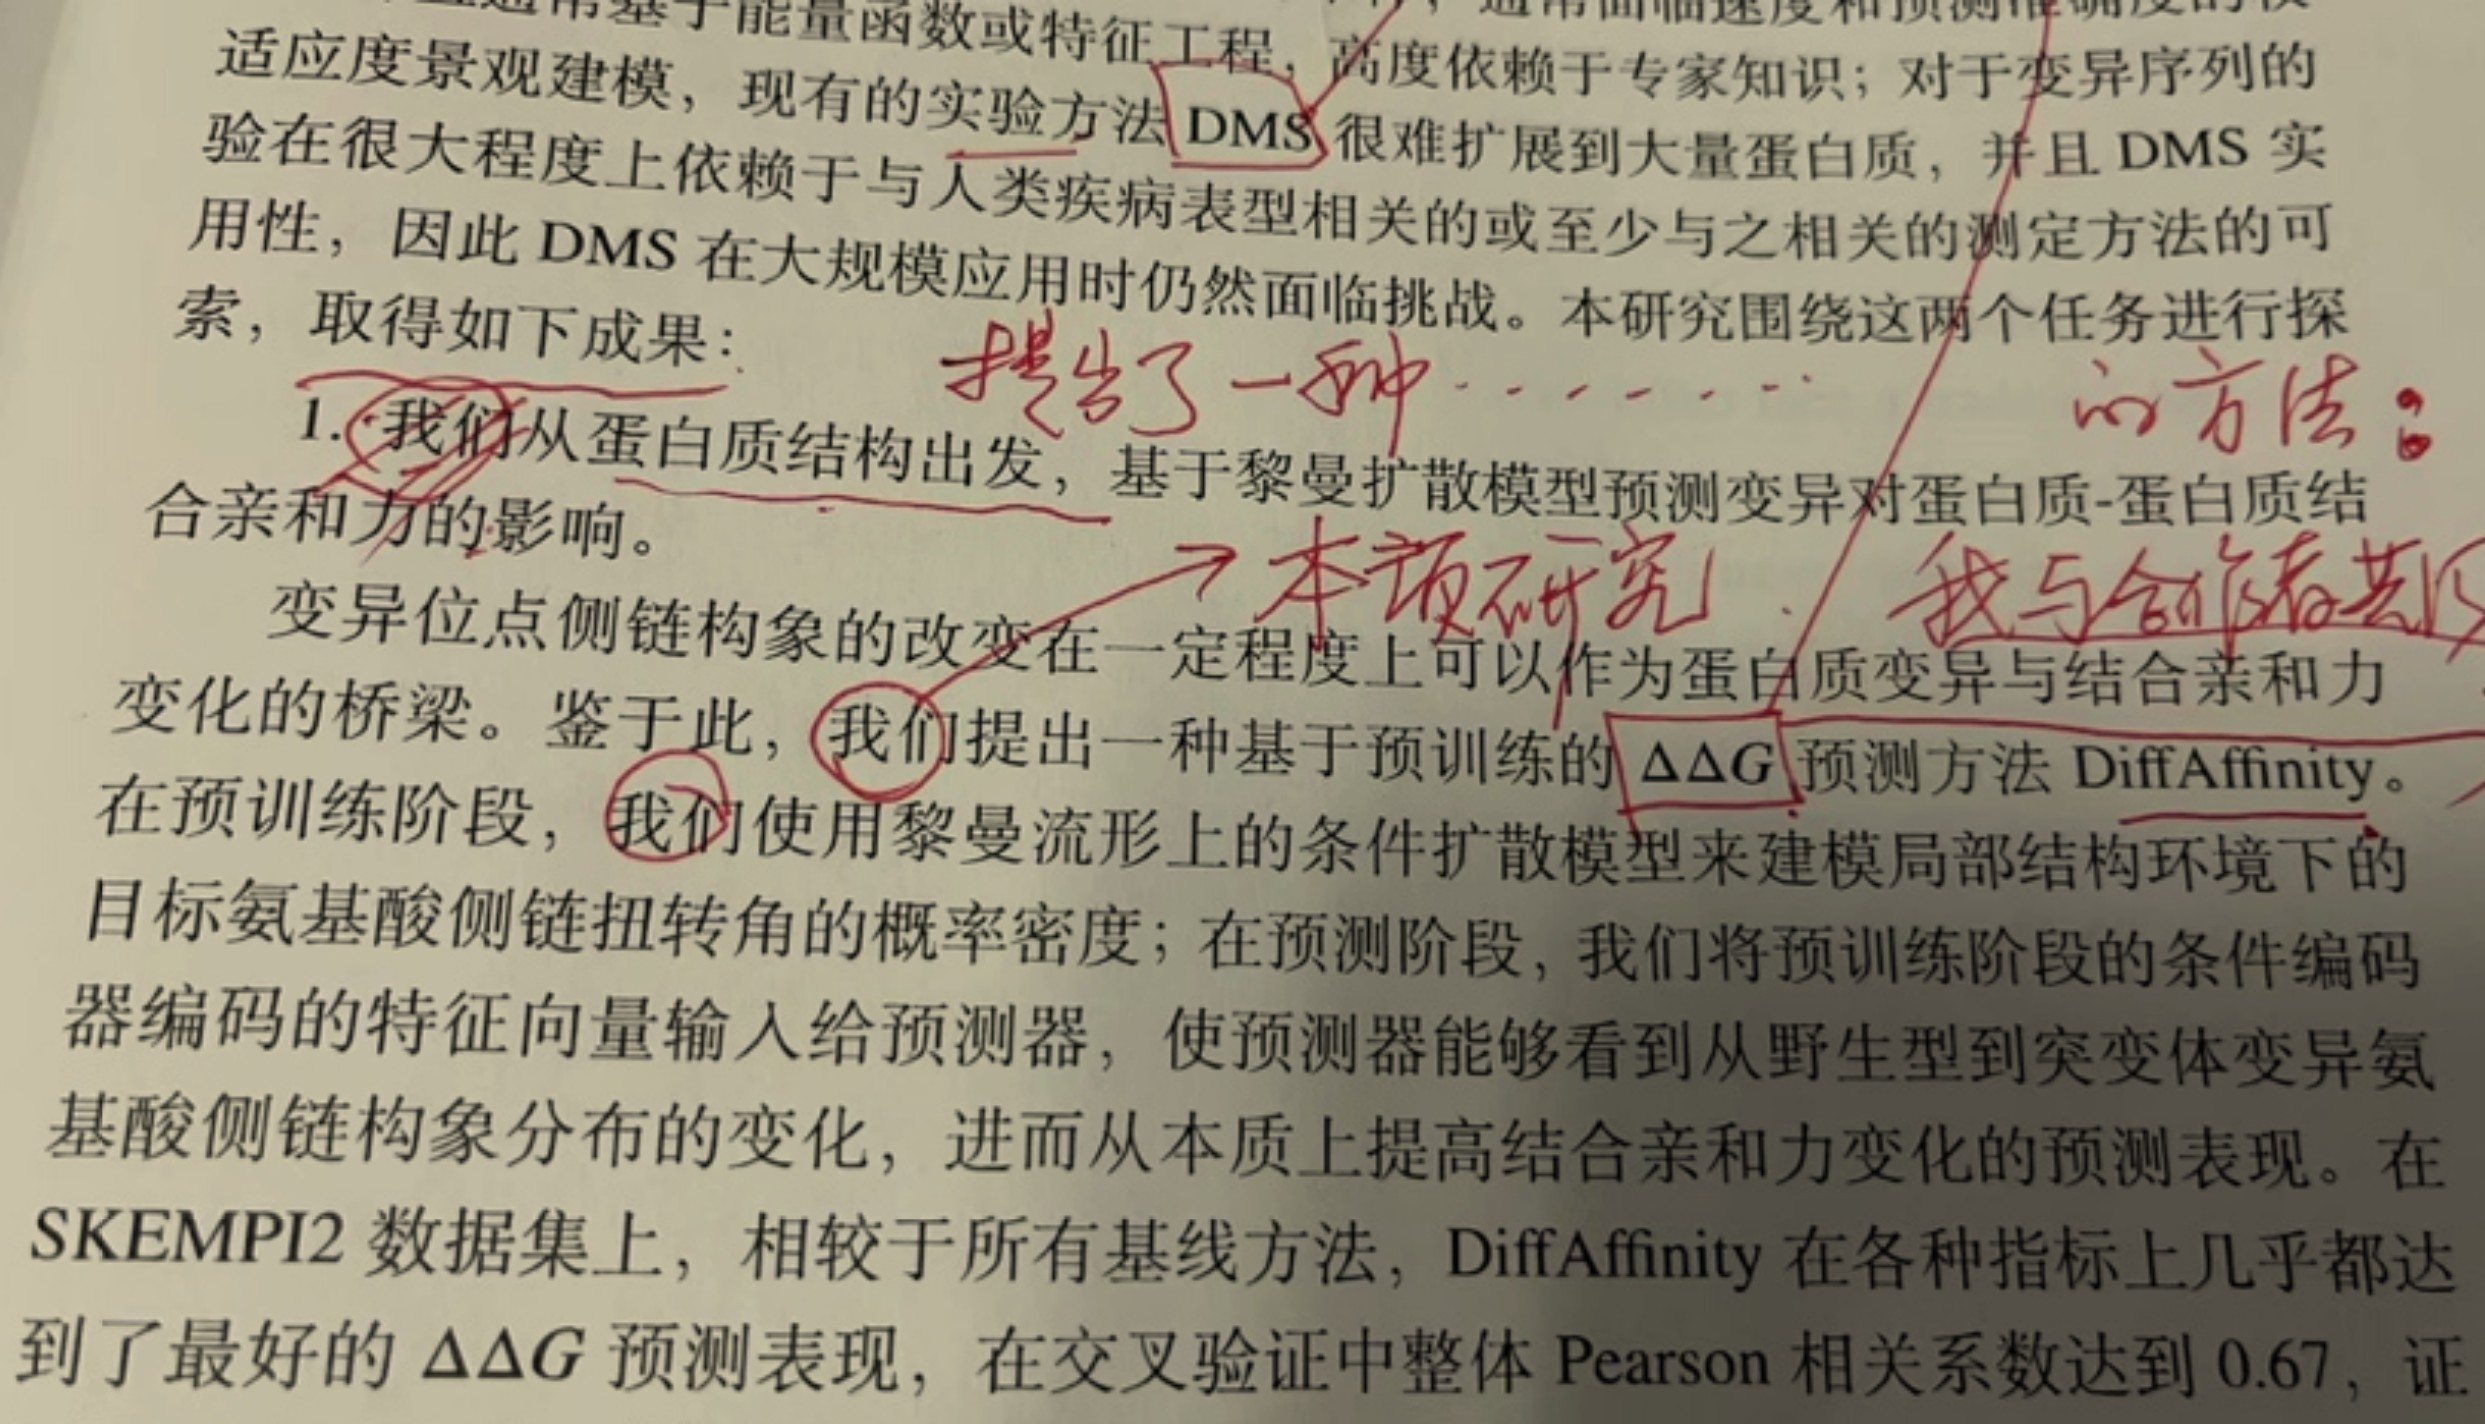
\includegraphics[scale=0.3]{doc/figures/chk01.jpg}
\caption{中文摘要错误之“我们”}
\label{fig:abstract-error-we}
\end{figure}

与期刊/会议论文(paper)不同,学位论文(thesis)是个人作品,供学位评定之用,因此具有浓厚的个人色彩。
为厘清其他个人或集体的贡献,学位论文中的前面都会包含一个声明,比如“学位论文系本人在导师指导下独立进行研究工作取得的成果;对本论文所涉及的研究工
作做出贡献的其他个人或集体,均已在文中以明确方式标明或致谢。”因此,在学位论文中陈述贡献时,不能用“我们”。关于这一点,剑桥大学专门写了一句话:
"For a dissertation with one author, do not use the "editorial we" in place of "I".The use of "we" by a single author is outrageously pretentious.".

解决方法:以“本文”或“本项研究”代替“我们”;在英文中,使用“Our research shows....”或“The conclusions made from this analysis are ....”替代“we”。

需要注意的是,这不是说通篇不能使用“我们”---“我们”有两层含义,一是表示“作者及其合作者”,即:“With the assistance of my colleagues, I designed …”,二是表示“作者和读者”,即:“the readers”。在采用第二个义项时,可以使用“我们”。


\item \emph{描述已完成工作时,建议采用如例\ref{examp:contribution-item}给出的“冒号式、分点陈述”格式,使用“提出了一种/开发了一套/构建了一个”等说法。}
\begin{figure}[!htpb]
\centering
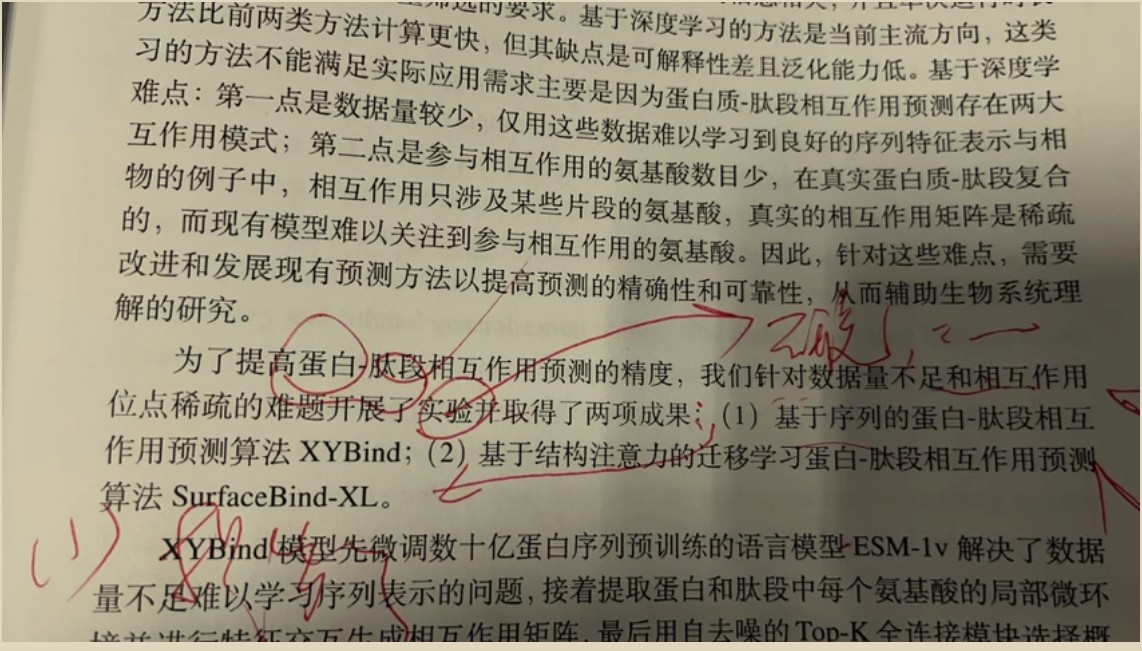
\includegraphics[scale=0.65]{doc/figures/chk02.jpg}
\caption{中文摘要错误之贡献分条列出}
\label{fig:abstract-error-contribution}
\end{figure}
\begin{example}\label{examp:contribution-item}
本项研究取得了如下成果:
\begin{enumerate}
    \item 提出了一种 xxxx 算法:详细陈述目标、基本思想、性能等。
    \item 设计了一个 xxx 系统:详细陈述目标、基本思想、性能等。
\end{enumerate}
\end{example}
\end{itemize}

\section{英文摘要}
英文摘要撰写注意事项:
(1) 尽量取消不必要的字句:如“It is reported…”,“The author discusses…”,“In this paper,”。 
(3) 采用短句叙述,但要避免句形单调;目的、方法、结果用过去时态,结论用一般现在时态;可用动词的情况应尽量避免用动词的名词形式;避免使用一长串形容词或名词来修饰名词;注意冠词用法,不要误用、滥用或随便省略冠词。
(4) 语言要精炼,多用简短、词义清楚、熟悉的词;避免使用文学性的描述手法撰写文摘。
(5) 对已经为大众所熟悉的缩写词可直接使用,对于那些仅为同行所熟悉的缩略语,应在题目、摘要或关键词中至少出现一次全称。
\begin{itemize}
\item \emph{英文摘要的题目常犯的毛病是叫“Research on xxx”,这是中文“关于xxx 的研究”的硬译,殊为不妥。哥伦比亚大学建议的规范写法是“A study of xxxx”,或者直接陈述贡献,如“Algorithms for xxxx”、“On the intractability of sequence assembly”。}
\end{itemize}


\section{关键词中的标点符号}
\begin{itemize}
\item \emph{关键词用逗号隔开;中文关键词用中文逗号分隔,英文关键词用英文逗号分隔}

关键词以显著的字符另起一行并隔行排列于摘要下方,左顶格,中文关键词间用中文逗号隔开\footnote{不同学校规定略有不同,比如清华大学规定学位论文中的关键词采用“;”分隔}。英文关键词应与中文关键词对应,首字母应大写,用英文逗号隔开。
\begin{enumerate}
\item 关键词编写一般包括论文审读、主题分析、选词和编排。
\item 关键词应准确并充分揭示论文主题内容,重要的可检索内容不应遗漏。
\item 根据学术论文研究的深度和广度,宜选择3~5个关键词。
\item 学术论文应编写英文关键词。
\item 重点审读题名、摘要、段落标题和结论等,必要时浏览重点章节和全文。
\item 不应仅依据题名进行主题分析
\end{enumerate}
\begin{figure}[!htpb]
\centering
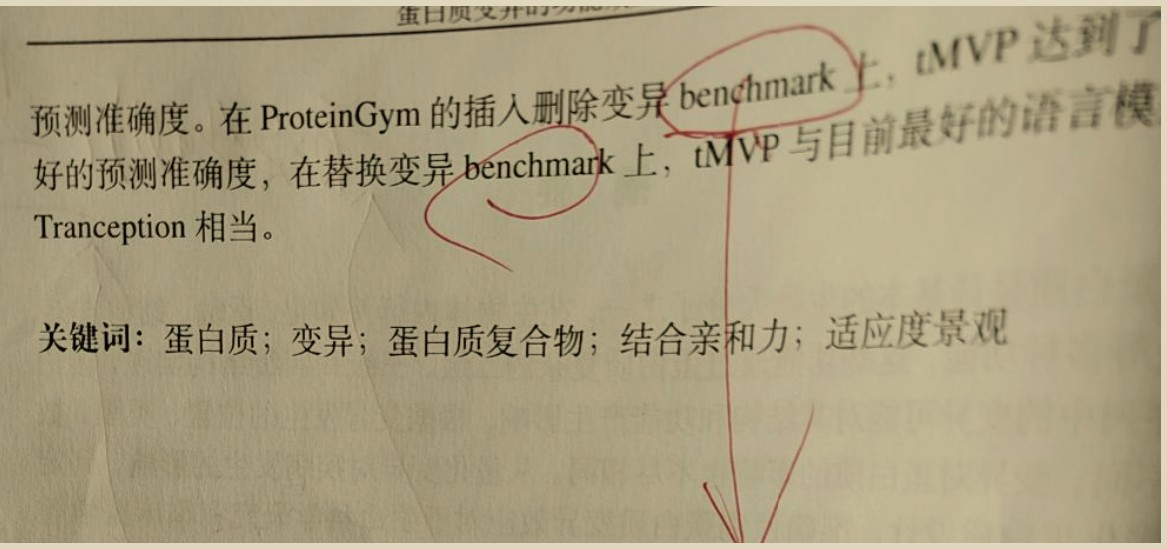
\includegraphics[scale=0.65]{doc/figures/chk05.jpg}
\caption{关键词分隔符}
\label{fig:keywords-sep}
\end{figure}
\end{itemize}





\section{英文缩写}
\begin{itemize}
\item \emph{首次出现英文缩写时,应采用“中文名(英文全称,缩写)”的格式;另,拉丁文要用斜体。比如大肠杆菌,应该写作“\textit{E. coli}”,中间有空格。}
\begin{figure}[!htpb]
\centering
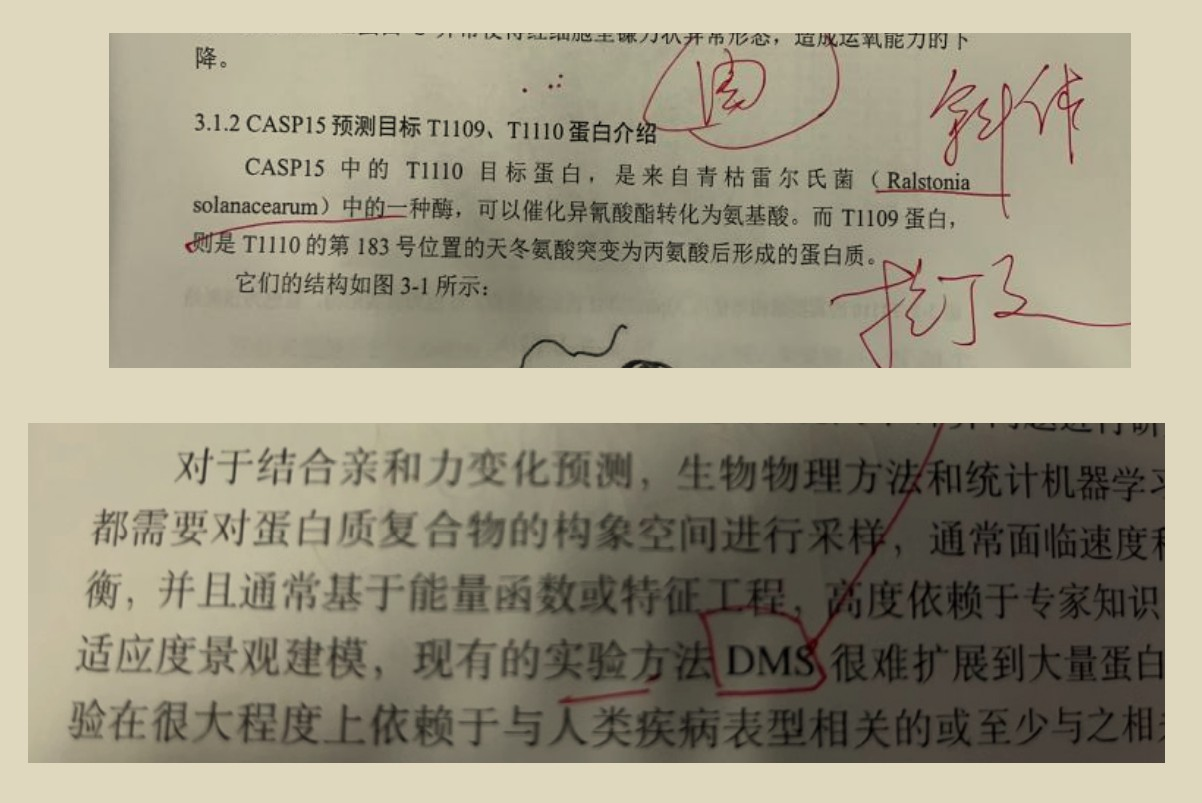
\includegraphics[scale=0.65]{doc/figures/chk03.jpg}
\caption{英文缩写格式错误}
\label{fig:abbrv-error}
\end{figure}
\end{itemize}

特殊名词或新名词应在适当位置加以说明或注解。双名法的生物学名部分均为拉丁文,并为斜体字。采用英语缩写词时,除本行业广泛应用的通用缩写词外,文中第一次出现的缩写词应该用括号注明英文原词。新的外来名词应用括号注
明英语全称和缩写语。



\section{中英文混杂}
\begin{itemize}
\item \emph{例如下图中的 benchmark,需要翻译成中文,不可中英混杂。另,常用的 Transformer 等都有规范译法。}
\begin{figure}[!htpb]
\centering
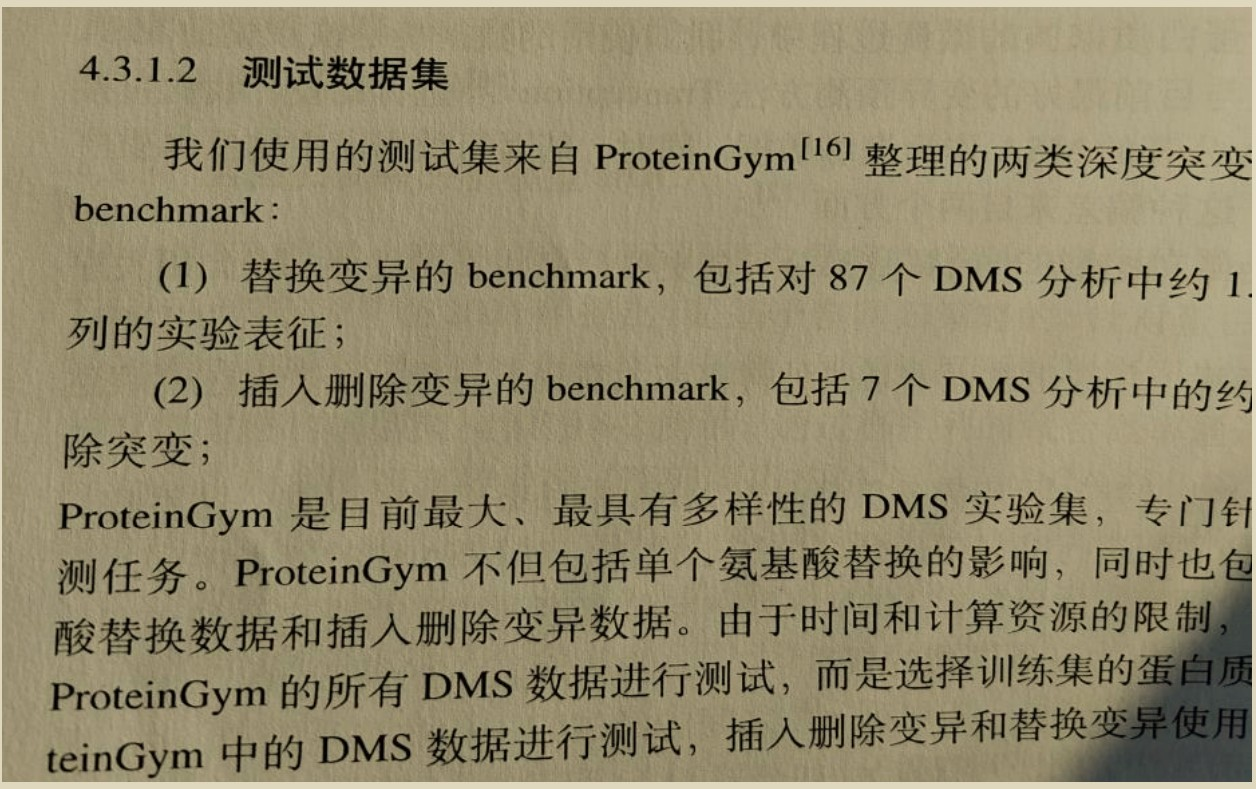
\includegraphics[scale=0.65]{doc/figures/chk04.jpg}
\caption{中英混杂错误}
\label{fig:mix-zh-cn-en-error}
\end{figure}
\end{itemize}




\section{避免含混}
不要出现易混淆词汇以及表示不明确句子。例如“序列”,讲清楚是“蛋白质序列”,不要以为读者靠上下文自然能够补足,要明确。再如“3.2.1 XYBind”中直接说 XYBind,读者会很糊涂;应该在前面加上“蛋白质-肽段相互作用预测算法 XYBind 的整体流程

\begin{figure}[!htpb]
\centering
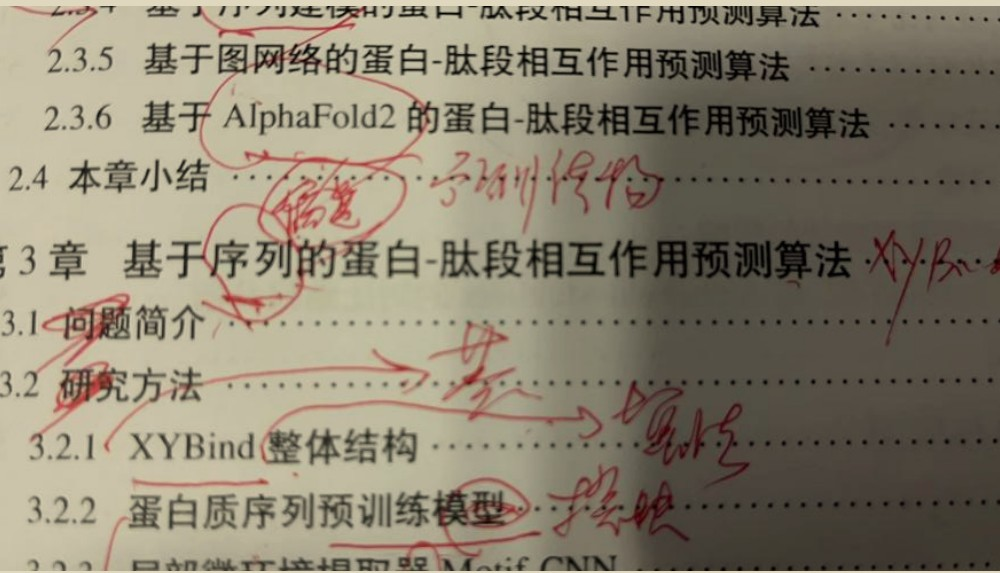
\includegraphics[scale=0.65]{doc/figures/chk06.jpg}
\caption{避免含混}
\label{fig:unclear-meanning}
\end{figure}


\section{公式排版}
\subsection{公式的转行}
关千数学式转行,1993年以前的国家标准没有做过明确的规定,大多数科技书刊在公式转行时遵循的是约定俗成的规则,即在 $=,+,-,/,\times,\cdot$ 等记号前转,并把这类记号放在下行行首。 

新标准对转行规则做出了明确的规定:“当一个表示式或方程式需要断开、用2行或多行来表示时,最好在紧靠其中记号$=,+,-,/,\times,\cdot,\pm$后断开,而在下一行开头不应重复这一记号。

读者看到上一行末尾的减号,就知道此式没有排完,下一行是由上一行转行来的,无论公式后面加不加点号,都不会产生误解。 这里的 “—”号,既是运算符号,又是连式符号,跟英文单词转行时需加的连字符所起的作用相同。至千转行的式子怎么排法,是居中排,还是与第1行的式子齐头,或是比第1行式子缩进几格;如果转行多次,转行的式子是否要左齐头排,或均居中排:新标准未作规定。 这些需要编辑根据版面设计要求和实际情况做出合理安排。




\subsection{公式的结尾}
数学式是用数字、字母和符号组合起来表达特定科学内容的,与文 字叙述具有同样的功能,是文章的有机组成部分。无论公式是串文排还 是居中排,在公式与公式之间,文字与公式之间,都要按实际需要确定 是否添加点号。公式尾部一定要加标点符号(英文)。如果公式所在的句子未结束,则使用逗号结尾,下一句不缩进;否则,以英文句号结尾,下一句要缩进。

下面的居中排公式后不应加点号:
\begin{example}
"……在比较一般的稳态黎曼时空
\begin{equation}
\mathrm{d} s^2 = g_{00} \mathrm{d} t^2  +  g_{11} \mathrm{d} x^2  +  g_{22} \mathrm{d} y^2  +  g_{33} \mathrm{d} z^2   +  2g_{03} \mathrm{d} t \mathrm{d} z  
\end{equation}
中,相对于视界……"
\end{example}

而下面的居中排公式后就需要加点号:
\begin{example}
"……式(XX)可写成
\begin{equation}
\hat{\rho} = \frac{1}{Z} \exp(-\beta ( \hat{H} - \Omega_{H} \hat{M})) \mbox{,}
\end{equation}
式中$\hat{H}$为……"
\end{example}


\subsection{公式 vs 程序}
公式就是公式,不能使用 Python 代码代替!

\begin{figure}[!htpb]
\centering
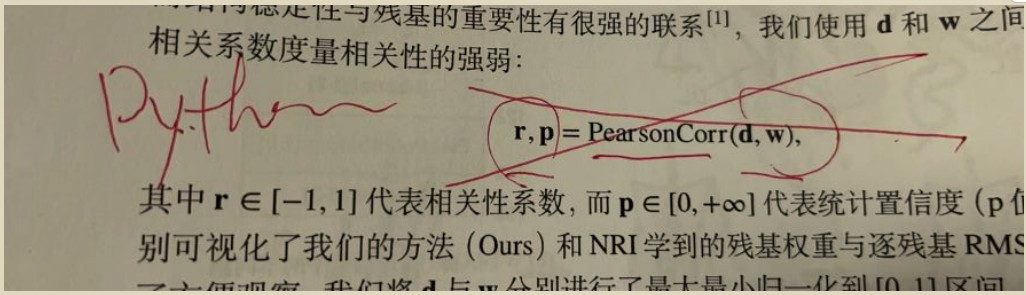
\includegraphics[scale=0.65]{doc/figures/chk08.jpg}
\caption{公式 vs 程序}
\label{fig:eqvscode}
\end{figure}


\section{表格}
表格的表头要用中文,不能用英文(如“Similarity”);数字一般情况下精确到小数点后 3 位,采用右对齐方式,以利于比较。

\section{图表的标题}
图表的标题要避免含混不清,不能指望读者从上下文猜测、补全出标题的含义,而应该是“含义自明的”,要突出与文章的关联;另,标题结尾不能出现标点符号。例如:图 2-3 的标题直接用“Social-LSTM”,比较突兀;应该前面加上短语以明示,比如改为“个体相互作用检查算法 Social-LSTM 中的社会力池化操作”,或者改成“基于……(社会力)模型……(任务)预测方法”。

各章标题中尽量不采用英文缩写词,对必须采用者,应使用本行业的通用缩写词,标题中尽量不使用标点符号。图应具有“自明性”,即只看图、图题和图注,不阅读正文,就可理解图意。每一图应有简短确切的图题,连同图序置于图下居中。


\chapter{附录功能测试}\label{appendix:testappfunc}

\section{数学环境测试}

\begin{axiom}
   这是一个公理。 
\end{axiom}
\begin{theorem}
   这是一个定理。 
\end{theorem}
\begin{lemma}
   这是一个引理。 
\end{lemma}
\begin{corollary}
   这是一个推论。 
\end{corollary}
\begin{assertion}
   这是一个断言。 
\end{assertion}
\begin{proposition}
   这是一个命题。 
\end{proposition}
\begin{proof}
    这是一个证明。
\end{proof}
\begin{definition}
    这是一个定义。
\end{definition}
\begin{example}
    这是一个例子。
\end{example}
\begin{remark}
    这是一个注。
\end{remark}

\section{数学公式测试}
\begin{equation} \label{eq:appedns-number}
    %\adddotsbeforeeqnnum%
    \begin{cases}
        \frac{\partial \rho}{\partial t} + \nabla\cdot(\rho\Vector{V}) = 0\\
        \frac{\partial (\rho\Vector{V})}{\partial t} + \nabla\cdot(\rho\Vector{V}\Vector{V}) = \nabla\cdot\Tensor{\sigma}\\
        \frac{\partial (\rho E)}{\partial t} + \nabla\cdot(\rho E\Vector{V}) = \nabla\cdot(k\nabla T) + \nabla\cdot(\Tensor{\sigma}\cdot\Vector{V})
    \end{cases}
    \nonumber
\end{equation}
\begin{equation}
    \adddotsbeforeeqnnum%
    \frac{\partial }{\partial t}\int\limits_{\Omega} u \, \mathrm{d}\Omega + \int\limits_{S} \unitVector{n}\cdot(u\Vector{V}) \, \mathrm{d}S = \dot{\phi}
    \nonumber
\end{equation}
\[
    \begin{split}
        \mathcal{L} \{f\}(s) &= \int _{0^{-}}^{\infty} f(t) e^{-st} \, \mathrm{d}t, \ 
        \mathscr{L} \{f\}(s) = \int _{0^{-}}^{\infty} f(t) e^{-st} \, \mathrm{d}t\\
        \mathcal{F} {\bigl (} f(x+x_{0}) {\bigr )} &= \mathcal{F} {\bigl (} f(x) {\bigr )} e^{2\pi i\xi x_{0}}, \ 
        \mathscr{F} {\bigl (} f(x+x_{0}) {\bigr )} = \mathscr{F} {\bigl (} f(x) {\bigr )} e^{2\pi i\xi x_{0}}
    \end{split}
\]

\section{测试公式编号 \texorpdfstring{$\Lambda,\lambda,\theta,\bar{\Lambda},\sqrt{S_{NN}}$}{$\textLambda,\textlambda,\texttheta,\bar{\textLambda},\sqrt{S_{NN}}$}} \label{sec:testmath}

\begin{equation} \label{eq:appedns}
    %\adddotsbeforeeqnnum%
    \begin{cases}
        \frac{\partial \rho}{\partial t} + \nabla\cdot(\rho\Vector{V}) = 0\\
        \frac{\partial (\rho\Vector{V})}{\partial t} + \nabla\cdot(\rho\Vector{V}\Vector{V}) = \nabla\cdot\Tensor{\sigma}\\
        \frac{\partial (\rho E)}{\partial t} + \nabla\cdot(\rho E\Vector{V}) = \nabla\cdot(k\nabla T) + \nabla\cdot(\Tensor{\sigma}\cdot\Vector{V})
    \end{cases}
\end{equation}
\begin{equation}
    %\adddotsbeforeeqnnum%
    \frac{\partial }{\partial t}\int\limits_{\Omega} u \, \mathrm{d}\Omega + \int\limits_{S} \unitVector{n}\cdot(u\Vector{V}) \, \mathrm{d}S = \dot{\phi}
\end{equation}
\[
    \begin{split}
        \mathcal{L} \{f\}(s) &= \int _{0^{-}}^{\infty} f(t) e^{-st} \, \mathrm{d}t, \ 
        \mathscr{L} \{f\}(s) = \int _{0^{-}}^{\infty} f(t) e^{-st} \, \mathrm{d}t\\
        \mathcal{F} {\bigl (} f(x+x_{0}) {\bigr )} &= \mathcal{F} {\bigl (} f(x) {\bigr )} e^{2\pi i\xi x_{0}}, \ 
        \mathscr{F} {\bigl (} f(x+x_{0}) {\bigr )} = \mathscr{F} {\bigl (} f(x) {\bigr )} e^{2\pi i\xi x_{0}}
    \end{split}
\]



%---------------------------------------------------------------------------% % appendix content

%--------------------------------------------------------------------
%-> Backmatter: cv, thanks
\backmatter% initialize the environment
%---------------------------------------------------------------------------%
%->> Backmatter
%---------------------------------------------------------------------------%
% --> 在读期间的成果
%
\begin{achievement}
%
%-->>A:在国内外刊物上发表的论文
\section*{A:在国内外刊物上发表的论文}

{
\begin{backitem}
\item Berger J O. Statistical decision theory and Bayesian analysis[M/OL]. second. New York, NY: Springer, 2010: 618. DOI: 10.1007/978-1-4757-4286-2.
\item Friston K. The free-energy principle: a unified brain theory?[J/OL]. Nature Reviews Neuroscience, 2010, 11(2): 127-138 [2020-11-27]. DOI: 10.1038/nrn2787.
\end{backitem}
}
%
%-->>B:在国际学术会议上发表的论文
\section*{B:在国际学术会议上发表的论文}

{
\begin{backitem}
\item Li J, Liu Y M, Chen H M, etal. A Pulsed Perturbation Facilitated Optical Optical Double Resonance Spectroscopy (PFOODR) Study of the High-Lying Electronic States of Na2. 13th International Conference on Laser Spectroscopy, Hangzhou, China, June 1997. (Invited Lecture)
\item Li J,Liu Y M, Ma H, et al. Dissociation of the Rydberg States of CaCl Investigated by Ion-dip Spectroscopy. 8th International Symposium on Resonance Ionization Spectroscopy and Its Applications, State College, Pennsylvania, USA, June 1995 .(Poster)
\end{backitem}
}
%
%-->>C:申请及授权专利 (无专利时此项不必列出)
\section*{C:申请及授权专利}
{
\begin{backitem}
\item 施金,张威,施敏,陈建新,曹青华,秦伟,包志华。一种用于天线的平衡式移相器,申请号:201710278510.9。授权时间:2019年7月26日。
\item 施金,聂怡,张威,徐凯,郁梅,张凌燕,李宏伟。一种平衡式滤波移相器,申请号:2020111661075。
\end{backitem}
}
%
%-->>D:所参加或主持的项目 (需标出项目编号、项目起始日期)(无项目时此项不必列出)
\section*{D:参加的项目}

{
\begin{backitem}
\item 南通市科技计划项目(项目编号:GY12016023; 项目名称:平衡式移相器设计)。主持并结题。
\item 江苏省高等学校自然科学研究面上项目(项目编号:17KJB510048; 项目名称:具有共模抑制的差分微波移相器关键技术研究)。参与。
\end{backitem}
}


\emph{(可以随意添加新的条目或是分节结构。)}


\end{achievement}





%---------------------------------------------------------------------------------
% - 致谢
%--> Acknowledgements

\begin{acknowledgment}
我走了很远的路,吃了很多的苦,才将这份博士学位论文送到你的面前。二十二载求学路,一路风雨泥泞,许多不容易。如梦一场,仿佛昨天一家人才团聚过。

出生在一个小山坳里,母亲在我十二岁时离家。父亲在家的日子不多,即便在我病得不能自己去医院的时候,也仅是留下勉强够治病的钱后又走了。我十七岁时,他因交通事故离世后,我哭得稀里糊涂,因为再得重病时没有谁来管我了。同年,和我住在一起的婆婆病故,真的无能为力。她照顾我十七年,下葬时却仅是一副薄薄的棺材。另一个家庭成员是老狗小花,为父亲和婆婆守过坟,后因我进城上高中而命不知何时何处所终。如兄长般的计算机启蒙老师邱浩没能看到我的大学录取通知书,对我照顾有加的师母也在不惑之前匆匆离开人世。每次回去看他们,这一座座坟茔都提示着生命的每一分钟都弥足珍贵。

人情冷暖,生离死别,固然让人痛苦与无奈,而贫穷则可能让人失去希望。家徒四壁,在煤油灯下写作业或者读书都是晚上最开心的事。如果下雨,保留节目就是用竹笋壳塞瓦缝防漏雨。高中之前的主要经济来源是夜里抓黄鳝、周末钓鱼、养小猪崽和出租水牛。那些年里,方圆十公里的水田和小河都被我用脚测量过无数次。被狗和蛇追,半夜落水,因蓄电瓶进水而摸黑逃回家中;学费没交,黄鳝却被父亲偷卖了,然后买了肉和酒,都是难以避免的事。

人后的苦尚且还能克服,人前的尊严却无比脆弱。上课的时候,因拖欠学费而经常被老师叫出教室约谈。雨天湿漉着上课,屁股后面说不定还是泥。夏天光着脚走在滚烫的路上。冬天穿着破旧衣服打着寒颤穿过那条长长的过道领作业本。这些都可能成为压垮骆驼的最后一根稻草。如果不是考试后常能从主席台领奖金,顺便能贴一墙奖状满足最后的虚荣心,我可能早已放弃。

身处命运的漩涡,耗尽心力去争取那些可能本就是稀松平常的东西,每次转折都显得那么身不由己。幸运的是,命运到底还有一丝怜惜,进入高中之后,学校免了全部学杂费,胡叔叔一家帮助解决了生活费。进入大学之后,计算机终于成了我一生的事业与希望,胃溃疡和胃出血也终与我作别。

从家出发坐大巴需要两个半小时才能到县城,一直盼着走出大山。从炬光乡小学、大寅镇中学、仪陇县中学、绵阳市南山中学,到重庆的西南大学,再到中科院自动化所,我也记不清有多少次因为现实的压力而觉得自己快抗不下去了。这一路,信念很简单,把书念下去,然后走出去,不枉活一世。世事难料,未来注定还会面对更为复杂的局面。但因为有了这些点点滴滴,我已经有勇气和耐心面对任何困难和挑战。理想不伟大,只愿年过半百,归来仍是少年,希望还有机会重新认识这个世界,不辜负这一生吃过的苦。最后如果还能做出点让别人生活更美好的事,那这辈子就赚了。

此致谢仅用作测试样例,其原作者为:\emph{中国科学院自动化研究所博士研究生 \quad 黄国平} 
\end{acknowledgment}




% other information
\cleardoublepage[plain]% 让文档总是结束于偶数页,可根据需要设定页眉页脚样式,如 [noheaderstyle]
\end{document}
\end{lstlisting}
%
\begin{enumerate}
\item \emph{制作标题} ~~ 命令 \verb|\maketitle| 定义了学位论文的扉页、学位论文原创性声明、学位论文使用授权声明和标题页。
\item \emph{目录}~~ 命令 \verb|\tableofcontents|自动生成学位论文的目录。
\item \emph{学位论文正文前事务处理}~~ 命令 \verb|\frontmatter| 格式化文档前的页面,覆盖中文摘要和英文摘要。文件"ntuthesis/Frontmatter.tex"中定义了学位论文的中文摘要和英文摘要。中文摘要由环境 \verb|\begin{abstract} ... ... \end{abstract}| 定义,中文关键词由命令 \verb|\keywords{}| 定义;英文摘要由环境 \verb|\begin{abstract*} ... ... \end{abstract*}| 定义,英文关键词由命令 \verb|\keywords*{}| 定义。 命令 \verb|\parwords{}| 定义中文段落关键词,相应地,命令 \verb|\parwords*{}| 定义英文段落关键词。
\item \emph{学位论文主体}~~ 命令 \verb|\mainmatter| 格式化文档主体页面,覆盖学位论正文各个章节、参考文献、缩略词表、综述、综述参考文献及附录各章节。
    \begin{itemize}
    \item 文件“ntuthesis/Mainmatter.tex”中定义了学位论文正文各个章节。
    \item 下列代码可以打印参考文献列表
        %\begin{lstlisting}[language=tex]
        \begin{verbatim}
        %reference matter
        {
            \intotoc*{\cleardoublepage}{\bibname}% add link to toc
            \linespread{1.25}
            \ntuthesisbibliography%{ref}
        }
        \end{verbatim}
        %\end{lstlisting}
    \item 缩略词表可以在文件"ntuthesis/Abbrvmatter.tex"中定义,缩略词表需要定义在环境 \verb|\begin{abbreviation} ... ... \end{abbreviation}|中,并且每个缩略词条目需要用命令 \verb|\addabbrvitem{<缩略词>}{<英文全称>}{中文}| 定义。
    \item 综述及综述文献写在文件"ntuthesis/Reviewmatter.tex"中。对于不需要综述及综述参考文献的,不包含该文件即可。该文件中,综述全文写在环境\verb|\begin{review} ... ... \end{review}|内,引用的参考文献bibtex索引信息写在正文的参考文献库即可。
    \item 命令 \verb|\appendix| 重定义附录章节计数格式,并初始化各个计数器。附录各个章节内容可以定义在文件"ntuthesis/Appendix.tex"中。
    \end{itemize}
    \item \emph{学位论文结尾事务处理}~~ 命令 \verb|\backmatter| 格式化学位论文尾部页面,覆盖在读期间的科研成果及致谢。这部分内容可以在文件"ntuthesis/Backmatter.tex"中定义。
        \begin{itemize}
        \item  在读期间学术成果写在环境 \verb|\begin{achievement} ... ... \end{achievement}| 中。在 \verb|achievement| 环境中,可以使用命令 \verb|\section*| 按学术成果类别分节列出,例如 \verb|\section*{A:在国内外刊物上发表的论文}| 、 \verb|\section*{B:在国际学术会议上发表的论文}| 、 \verb|\section*{C:申请及授权专利}| 、 \verb|\section*{D:参加的项目}| 等。在每个分节中需要添加一个环境 \verb|\begin{backitem} ... ... \end{backitem}|,并且使用命令 \verb|\item| 逐条添加。 每个条目的格式需要满足文献引用格式要求。可以随意添加新的条目或是分节结构。\emph{此部分仅适用于研究生,本科毕业设计不需要此部分!}
        \item 致谢写在环境 \verb|\begin{acknowledgment} ... ... \end{acknowledgment}| 中。不需要写签名,会自动生成结尾签名。
        \emph{本科毕业设计的致谢部分归入} \verb|\mainmatter| \emph{命令范围内,正常使用即可!}
        \end{itemize}
        
    \item 命令 \verb|\cleardoublepage[plain]| 通过添加空白页方式强制学位论文以偶数页结束。 
\end{enumerate}